\documentclass[12pt,a4paper,leqno]{article}

\usepackage[utf8]{inputenc}
\usepackage[T1]{fontenc}
\usepackage[english]{babel}
\usepackage{amsthm}
\usepackage{amsfonts}         
\usepackage{amsmath}
\usepackage{amssymb}
\usepackage{mathrsfs}
\usepackage{hyperref}
\usepackage[all]{hypcap}
\usepackage{tikz}
\usepackage{float}
\usepackage{placeins}
\usepackage{afterpage}
\usetikzlibrary{matrix, arrows, decorations.pathmorphing}
\DeclareMathAlphabet{\mathpzc}{OT1}{pzc}{m}{it}

\newcommand{\R}{\mathbb{R}}
\newcommand{\C}{\mathbb{C}}
\newcommand{\Q}{\mathbb{Q}}
\newcommand{\N}{\mathbb{N}}
\newcommand{\Aff}{\mathbb{A}}
\newcommand{\Proj}{\mathbb{P}}
\newcommand{\No}{\mathbb{N}_0}
\newcommand{\Z}{\mathbb{Z}}
\newcommand{\OO}{\mathcal{O}}
\newcommand{\diam}{\operatorname{diam}}

\newcommand{\cat}{\mathcal}
\newcommand{\isomto}{\stackrel{\sim}{\rightarrow}}
\newcommand{\coker}{\mathrm{coker}}
\newcommand{\im}{\mathrm{im}}
\newcommand{\coim}{\mathrm{coim}}
\newcommand{\spec}{\mathrm{Spec}}
\newcommand{\gr}{\mathrm{gr}}
\newcommand{\plim}{\varprojlim}
\newcommand{\dlim}{\varinjlim}
\newcommand{\bl}{\mathrm{Bl}}
\newcommand{\proj}{\mathrm{Proj}}
\newcommand{\rproj}{\mathpzc{Proj}}
\newcommand{\supp}{\mathrm{supp}}
\newcommand{\cosupp}{\mathrm{cosupp}}
\newcommand{\der}{\mathrm{Der}}
\newcommand{\Ex}{\mathrm{Ex}}

\newcommand{\sectionbreak}{\clearpage}

\newcommand{\fref}[1]{\hyperref[{#1}]{\ref*{#1}}}


\newtheorem{theo}{Theorem}[section]
\theoremstyle{plain}
\newtheorem{thm}[theo]{Theorem}
\newtheorem{lem}[theo]{Lemma}
\newtheorem{prop}[theo]{Proposition}
\newtheorem{cor}[theo]{Corollary}

\theoremstyle{definition}
\newtheorem{defn}[theo]{Definition}
\newtheorem{con}[theo]{Conjecture}
\newtheorem{ex}[theo]{Example}

\theoremstyle{remark}
\newtheorem{rem}[theo]{Remark}

\pagestyle{plain}
\setcounter{page}{1}
\addtolength{\hoffset}{-1.15cm}
\addtolength{\textwidth}{2.3cm}
\addtolength{\voffset}{0.45cm}
\addtolength{\textheight}{-0.9cm}

\title{Resolution of Singularities}
\author{Toni Annala}
\date{}

\begin{document}

\maketitle

\tableofcontents

\section{Introduction}

For many of the most important theorems in mathematics giving even an approximate idea of what the theorem states is fairly hard. This is not the case with resolution of singularities. The basic idea is very geometric, and can be easily stated approximately assuming very little prior mathematics background. It is a statement considering varieties, i.e., solution sets of equation systems consisting entirely of polynomial equations.

Let us start with an example. The solution set for the equation $y^2 - x^3$ is visualized in Figure \fref{cusp1}. At every point of the curve, except at the origin, the curve seems to be smooth, i.e., if we zoom close enough, it starts looking like a straight line. These kind of points are called \emph{nonsingular} or \emph{regular points}. More generally in higher dimensional varieties (say the dimension is $n$) we would consider a point to be nonsingular if locally around it the variety looks like the ''normal'' $n$-dimensional space (you can think of $\R^n$ if we are dealing with real solutions, $\C^n$ if with complex solutions).  

\begin{figure}[!htbp]\label{cusp1}
\begin{center}
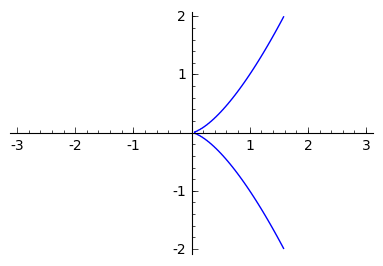
\includegraphics{pics/cusp.png}
\caption{A cusp.}
\end{center}
\end{figure}

Something weird happens at the origin: the direction of the curve ''changes'' suddenly, and no matter how close we try to zoom, the curve will never start looking like a straight line. Points that fail to be nonsingular are called \emph{singularities} or \emph{singular points}. The type of curve singularity we have in Figure \fref{cusp1} is called a \emph{cusp}.

Now a question arises: would it be possible to parametrize our singular curve $C$ with another, nicer, curve: could we parametrize the points of $C$ with points of a nonsingular curve $C'$ (meaning that it has no singular points)? In the above case it is indeed possible. Take the curve $C'$ that is the zero set of the polynomial equation $y'^2 - x'$ plotted in Figure \fref{nsing1}. We would like to define a map $C' \to C$. Send a point $(x',y') \in C'$ to $(x',y'x')$. This point lies in $C$ as
\begin{align*}
\left( y'x' \right) ^ 2 - x'^3 = x'^2 (y'^2 - x'),
\end{align*}
and the right hand side is zero by assumption. Hence we have what we desired: a parametrization of the curve $C$ by a nonsingular curve $C'$.

\begin{figure}[!htbp]\label{nsing1}
\begin{center}
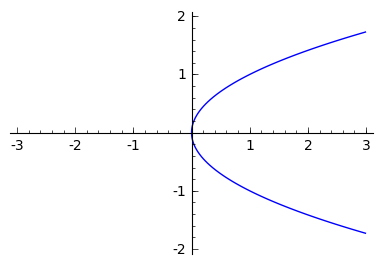
\includegraphics{pics/parabola.png}
\caption{The solution set for $y'^2 - x' = 0$.}
\end{center}
\end{figure}

\begin{figure}[!htbp]\label{node1}
\begin{center}
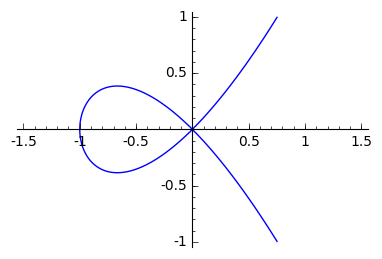
\includegraphics{pics/node.png}
\caption{This kind of singularity is called a \emph{node}.}
\end{center}
\end{figure}

Before going further, let us have another example. The equation $y^2 - x^3 - x^2$ gives the curve visualized in Figure \fref{node1}. The origin is clearly singular, but this singularity is different from the one we had in Figure \fref{cusp1}. The curve intersects itself! Luckily this self-intersection is in some sense as good as possible, at least the different branches meet \emph{transversally}, i.e., they have distinct tangent lines. A singular point, where two branches of a curve meet transversally is called a \emph{node}. 

Can we find a nonsingular parametrization for this curve? Yes we can. Take the curve $y'^2 - x' - 1$, which is visualized in Figure \fref{nsing2}. A parametrization is again given by $(x', y') \mapsto (x', x'y')$ which can be checked with similar reasoning as before.


\begin{figure}[!htbp]\label{nsing2}
\begin{center}
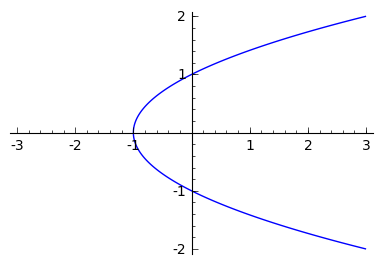
\includegraphics{pics/parabola2.png}
\caption{I swear, the resolved curve won't \emph{always} be a parabola.}
\end{center}
\end{figure}

Finding a parametrization of a singular variety by a nonsingular one is called \emph{resolving} its singularities (this is not what one usually means by it, usually we would require the parametrizing curve to be isomorphic to the original one almost everywhere). The problem of resolution of singularities simply asks whether or not the singularities of any variety can be resolved. 

\subsection{A condenced historical account of the problem}

Although the problem is much older, we start with the work of Oscar Zariski. He was arguably the leading algebraic geometer of the first half of the twentieth century: if Grothendieck is to be regarded as the father of modern algebraic geometry, then Zariski must surely be the grandfather. After doing his undergraduate studies in Kiev, the unstable political atmosphere drove him out of the country, and he left for Rome, where he pursued his doctorate under the leading algebraic geometers of his time. This is what is nowdays known as the Italian school of classical algebraic geometry. By using ''geometric intuition'' they pushed algebraic geometry forward to new and exciting directions, but unfortunately the lack of rigour caused them to publish some untrue theorems, and nowdays they serve (somewhat unjustly) as some kind of example of what can happen when you disregard rigour.

Zariski was originally interested in algebra, and was algebraically inclined than his Italian teachers. And even though he enjoyed the geometric way of thinking of the Italians, he also had some worries concerning the rigour of their arguments. Because of these reasons, Castelnuovo, his advisor, once stated: ''Zariski, you are here with us but are not one of us'' \cite{Par}. This was not meant in a bad way, the methods of the Italian school had reached a dead-end, and would no longer be able to accomplish significant progress in the field, and Castelnuovo knew this all too well. But it would still take years before Zariski would start systematically rebuilding the foundations of algebraic geometry.

In 1932, now in the United States, Zariski began to work on his monograph \emph{Algebraic Surfaces}, a task that would take him three years. The purpose of the monograph was to give a complete account of the results concerning algebraic curves obtained by the Italian school with rigorous proofs. However, while writing the book, he became increasingly certain that the entire foundations of algebraic geometry should be completely rebuilt using commutative algebra. He later stated himself: ''working on that book took all my time because as I worked I became more and more disgusted with the kind of proofs that the Italian geometers were giving, and I started studying algebra seriously.'' \cite{Par} He started incorporating recent results from commutative algebra achieved by Noether, Krull and Dedekind, and casting everything in algebraic geometry in terms of the theory of commutative rings and their ideals. 

After the completion of the monograph in 1935, Zariski went on to develop an abstract theory of algebraic geometry over an arbitrary (algebraically closed) ground field (instead of the coordinates of the points being complex numbers, they could be elements of some abstract field). It was during this time when he got interested in the resolution problem. The problem of resolution of singularities for higher dimensional varieties had long stood open, and many good mathematicians had given it a shot. Nonetheless, only some partial results had been achieved, and these were over complex numbers.

Zariski gave a simple proof for the resolution problem for surfaces using his notion of \emph{normalization}, a term that should ring a bell to anyone who has studied algebraic geometry or commutative algebra. Resolution for surfaces is more complicated than for curves as the singularities of a surface need not to be confined in a finite set of points: the singular points can form curves as well. Normalizing a variety produces a variety whose singularities are of codimension two, which, in the case of surfaces, means that all singularities are point-singularities, i.e., the earlier complication is now gone! After normalization, resolving the remaining singularities is fairly straightforward.

The resolution of singularities for surfaces had, however, essentially already been solved by the Italian algebraic geometers \cite{Par}. But Zariski didn't stop there. Later, he was able to show that the singularities of three-folds over a field of characteristic zero (three dimensional varieties) can be resolved. This was a problem that had completely eluded the approaches of the Italian school, and was also the moment that proved to rest of the world how powerful the new algebraic methods Zariski had introduced could be.

This is however where the contributions of Zariski (essentially) end. For further progress some time had to pass, and another rebuilding of the foundations of algebraic geometry had to happen. Alexander Grothendieck, motivated by the famous Weil conjectures linking together number theory and geometry, began a systematic rebuilding of the whole field in mid 50s. The result was a very powerful theory of algebraic geometry, whose level of abstraction was something previously unseen in mathematics. Even Mumford, a student of Zariski who won the Fields medal in 1974, stated the following in a letter to Grothendieck: ''... I should say that I find the style of the finished works, esp. EGA, to be difficult and sometimes unreadable, because of its attempt to reach superhuman level of completeness.'' \cite{Mum} One can only imagine the struggle for those mathematicians that weren't quite as good as Mumford when trying to learn the theory. Such was the power of this theory, however, that the theory became universally accepted rather quickly, and is nowadays the standard way of doing algebraic geometry.

At the time, resolution of singularities was considered one of the most important open problems in algebraic geometry, for it would enable one to transfer many questions concerning singular varieties to questions involving only nonsingular ones, which are better understood. Even Grothendieck considered the problem to be one of the two most important ones, alongside his \emph{standard conjectures} (which, to this day, remain open).

In the 60s Heisuke Hironaka, another student of Zariski to be given the Fields medal, decided to attack the resolution problem. Zariski himself never truly tried to deploy the Grothendieck style of algebraic geometry. This was probably due to the great time investment required in order to learn to use it, combined with the fact that his own research was going well enough without the new tools. \cite{Par} But Hironaka, like many of the students of Zariski, fully endorsed this new theory. With the new tools given by the theory of schemes, he was able to do what Zariski himself had tried and failed: in the famous paper published in 1964 in Annals of Mathematics, Hironaka gave a complete proof for resolution of singularities over a ground field of characteristic zero. 

The proof, originally around 200 pages long, quickly gained a reputation for being extremely complicated and hard to understand. However, in further research the proof has been simplified and shortened considerably. For example in \cite{Wlo} W\l{}odarczyk gives a self contained proof for resolution of singularities via a Hironaka-style argument in just around twenty pages! An overview of a Hironaka-style argument for proof of resolution of singularities in characteristic 0 is given in Section \fref{HirRes}.

This still left open the finite characteristic case important in many applications to number theory. Partial results were obtained by Shreeram Abhyankar, another student of Zariski, who in 1966 published a proof for resolution of singularities for three-folds over algebraically closed fields of finite characteristic different from $2,3$ and $5$ \cite{HLOQ}. He later on went to generalize his result for three-folds in characteristic $2,3$ and $5$, as well as giving a proof for resolution of singularities for arithmetic surfaces.

However, for a long time essentially no progress was made. Hironaka's argument resisted all attempts of generalization to finite characteristic, and all algebraic approaches in the spirit of Zariski and his students seemed to fail as well. The initial success of the algebraic approach had blinded almost the entire field into thinking that this was the right way. The spell was finally broken by a young Dutch mathematician Aise Johan de Jong, who in a 1995 talk gave an outline for a very geometric proof for resolving singularities by means of so called alterations. 

His proof, published in a 1996 article \cite{Jong}, worked just as well over finite characteristic. A circle had closed: first algebra had had to replace geometry when geometrical methods failed, and now geometry, when all algebraic approaches seemed to fail, replaced algebra. Perhaps the most striking trait of his proof was the fact that essentially everything needed was already well known for nearly twenty years before the proof \cite{HLOQ}, the ingenious part was how the results were put together.

The resolution given by alterations is not, however, a resolution in the traditional sense. Traditionally one wants the resolution to produce a variety that is \emph{birational} to the original variety, i.e., it is isomorphic to the original variety outside some small subset. What de Jongs method gives is more like some kind of finite cover. But for many of the applications this is enough. The traditional problem of resolution of singularities in finite characteristic remains open.


\section{Completions}

This section is devoted to an important construction called \emph{completion} which, together with localization, forms a very powerful way of looking at the structure of an algebraic variety near a point. Familiarity with basic algebraic geometry and commutative algebra is assumed.

We begin with a motivating example. Recall the nodal curve $C$ from the first section, defined as the solution set of the polynomial $y^2 - x^3 - x^2$. At the origin the curve intersects itself, and it seems like the curve should, at least near the origin, consist of two components. But as $y^2 - x^3 - x^2$ is an irreducible polynomial, the coordinate ring $\OO_C (C)$ is an integral domain, as is the localization $\OO_{C,p}$ at origin $p$.

\begin{figure}[!htbp]\label{node2}
\begin{center}
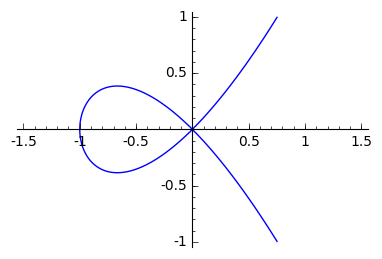
\includegraphics{pics/node.png}
\caption{The nodal curve.}
\end{center}
\end{figure}

This can be thought in the following way. The open sets of the Zariski topology are just the curve $C$ minus finitely many points, so they contain almost all of the curve $C$. The localization at origin gives essentially all information about the curve $C$ found in arbitrarily small neighbourhoods of the origin, and as none of these is small enough to make $C$ irreducible, the localization stays irreducible. It is as if algebra doesn't allow us to see close enough.

Of course analytically we may break the curve into to branches: the equation of the curve
\begin{equation*}
y^2 = x^3 + x^2
\end{equation*}
can be solved to give
\begin{equation*}
y = \pm \sqrt{x^3 + x^2} =  \pm x \sqrt{1+x},
\end{equation*}
describing the two branches of the curve.

We may connect this back to algebraic geometry when we note that $\sqrt{1+x}$ can be expressed by its Taylor series. Hence, if we think $y^2 - x^3 - x^2$ as an element of the formal power series ring $k[[x,y]]$ instead of the polynomial ring $k[x,y]$, the equation $y^2 - x^3 - x^2$ cuts out a reducible subscheme of $\spec k[[x,y]]$, and the irreducible components correspond to the two branches at the origin. Somehow, when we passed into the ring of formal power series, we are now much closer to the origin than by localization. 

As $k[[x,y]]$ is a local ring with maximal ideal $(x,y)$, the localization $k[x,y]_{(x,y)}$ embeds into it, and from this it is fairly easy to see that $\OO_{C,p}$ embeds into $k[[x,y]]/(y^2 - x^3 - x^2)$. The idea of completion of local rings is exactly this: we want to get closer, so instead of just looking at the localization, we somehow replace the local ring with some sort of power series ring. We say that we pass into \emph{formal neighbourhood} of a point $p$ when we do this. The nice thing is that these are usually much simpler than the local rings: for example, if we have a nonsingular $k$-variety $X$ of dimension $d$, where $k$ is algebraically closed, then the completion $\widehat \OO_{X,p}$ of the local ring at a closed point $p$ is isomorphic to $k[[x_1,...,x_d]]$.

\subsection{Completion of topological abelian groups}

Let $G$ be a topological abelian group. We say that a sequence $(x_i)$ in $G$ is \emph{Cauchy sequence} if for all neighbourhoods $U$ of $0$ we have $N_U \in \N$ such that $x_i - x_j \in U$ for all $i,j \geq N_U$. We say that $G$ is \emph{complete} if all Cauchy sequences converge to some value in $G$. Although this notion does make sense for non-Hausdorff groups too, from now on we will require complete groups to be Hausdorff.

Before continuing, we quickly recall the following useful fact of topological groups. If we set $U_0$ to be the intersection of all neighbourhoods of 0, then it is in fact true that $U_0$ is a subgroup of $G$. Moreover, this subgroup is closed, and it is zero if and only if $G$ is Hausdorff. The topological group $G / U_0$ is Hausdorff and $U_0$ is contained in the kernel of any continuous homomorphism $G \to H$, where $H$ is Hausdorff.

\begin{defn}
Let $G$ be a topological abelian group. The \emph{(Hausdorff) completion} of $G$, denoted by $\widehat G$, is ''the smallest complete group where $G$ can be mapped into''. More precisely, this means that completion is a continuous group morphism $G \to \widehat G$, where $\widehat G$ is complete, and for all continuous homomorphisms $G \to X$, where $X$ is complete, we have a unique morphism such that the following diagram commutes:

\begin{center}
\begin{tikzpicture}[scale=1]
\node (G) at (0,0) {$G$};
\node (Ghat) at (0,2) {$\widehat G$};
\node (X) at (3,2) {$X$};


\path[]
(G) edge[->] (Ghat)
(G) edge[->] (X)
(Ghat) edge[->, dashed] node[above]{$\exists !$} (X)
;
\end{tikzpicture}
\end{center}
It is clear that this defines $\widehat G$ up to unique isomorphism if it exists. Given a continuous homomorphism $f: G \to H$, the universal property induces a morphism $\widehat f : \widehat G \to \widehat H$, and it is easy to check that this defines a functor.
\end{defn}

First property of the completion we are going to prove is the fact that it commutes with ''passing into Hausdorffication''.

\begin{prop}
Let $G$ be a topological abelian group and $U_0$ the intersection of all neighbourhoods of $0$. If the completion of $G/U_0$ exist, then $G \to G/U_0 \to \widehat{(G/U_0)}$ is the completion of $G$.
\end{prop}
\begin{proof}
Assume we have a morphism $G \to X$, where $X$ is a complete topological group. As $X$ is Hausdorff, we know that $U_0$ is contained in the kernel of our map, and we can find a unique morphism $G / U_0 \to X$ making the diagram
\begin{center}
\begin{tikzpicture}[scale=1]
\node (G) at (0,0) {$G$};
\node (GH) at (0,2) {$G/U_0$};
\node (X) at (3,0) {$X$};

\path[]
(G) edge[->] (GH)
(G) edge[->] (X)
(GH) edge[->, dashed] node[above]{$\exists !$} (X)
;
\end{tikzpicture}
\end{center}
commute. We can now use the fact that the completion of $G / U_0$ is known to exist, and hence we have a unique map $\widehat {(G/U_0)} \to X$ making the upper triangle of
\begin{center}
\begin{tikzpicture}[scale=1]
\node (G) at (0,0) {$G$};
\node (GH) at (0,2) {$G/U_0$};
\node (X) at (3,0) {$X$};
\node (GHh) at (3,2) {$\widehat{(G / U_0)}$};

\path[]
(G) edge[->] (GH)
(G) edge[->] (X)
(GH) edge[->] (GHh)
(GHh) edge[->,dashed] node[right]{$\exists !$} (X)
(GH) edge[->] (X)
;
\end{tikzpicture}
\end{center}
commute. As $G \to G/U_0$ is surjective, the map $\widehat {(G/U_0)} \to X$ is also the only one making
\begin{center}
\begin{tikzpicture}[scale=1]
\node (G) at (0,0) {$G$};
\node (Ghat) at (0,2) {$\widehat {(G/U_0)}$};
\node (X) at (3,2) {$X$};


\path[]
(G) edge[->] (Ghat)
(G) edge[->] (X)
(Ghat) edge[->, dashed] node[above]{$\exists !$} (X)
;
\end{tikzpicture}
\end{center}
commute, and hence we are done.
\end{proof}

Next we will show that the completion always exists when $G$ is first countable. The idea is exactly the same one that is used when completing metric spaces.

Denote by $s(G)$ the set of Cauchy sequences in group $G$. This is a group: if $(x_i)$ is a Cauchy sequence, then so is $(-x_i)$ for negation is homeomorphism. If $(x_i)$ and $(y_i)$ are Cauchy sequences, then so is $(x_i + y_i)$. This is not too hard to see: for all neighbourhoods $U$ of the origin, we have smaller neighbourhoods $V_1$ and $V_2$ such that $V_1 + V_2 \subset U$ by continuity of summation. Then we may choose $N$ to be large enough so that $x_i-x_j \in V_1$ and $y_i-y_j \in V_2$ for all $i,j \geq N$. Now $(x_i + y_i) - (x_j + y_j) = (x_i - x_j) + (y_i - y_j) \in U$. Similarly we can see that $s_0(G)$, the sequences of $G$ that converge to 0, is a subgroup of $s(G)$. We define a topological group $G'$ algebraically as $s(G) / s_0(G)$.

Next we define $G'$ topologically. For every neighbourhood $U$ of 0, let $U' \subset G'$ consist of those equivalence classes $[(x_i)]$ for which there exists a neighbourhood $\epsilon$ of origin, such that $x_i + \epsilon \subset U$ for $i \gg 0$. This is clearly independent of the choice of the representative $(x_i)$. This forms a neighbourhood basis for $0$ in $G'$ inducing a structure of a topological group, as the next lemma shows. 

\begin{lem}\label{TopGroupFromNbhd}
The open sets $U'$ define a structure of a topological group on $G'$ when we give $G'$ the topology where the open sets are of form
\begin{equation*}
\{O \subset G \mid \mathrm{for \ all \ } x \in G \mathrm{\ we \ have \ } U' \mathrm{\ s.t. \ } x+U' \subset O \}.
\end{equation*}
In this topology $U'$ form a neighbourhood basis for $0$ (we do not yet claim these to be open, although it is true).
\end{lem}
\begin{proof}
From basic properties of topological groups, it suffices to show that the following three properties hold:
\begin{enumerate}
\item For all $U',V'$ we have $W'$ such that $W' \subset U' \cap V'$.
\item For all $U'$ we have $V'$ such that $V'+V' \subset U'$.
\item For all $U'$ we have $V'$ such that $V' \subset -U'$.
\end{enumerate}
Verifying these conditions is fairly straightforward:

\begin{enumerate}
\item Here we may take $W = U \cap V$. For if $x \in W'$, then for some $\epsilon$ we have that $x_i + \epsilon \subset W$ for $i$ large enough, and hence also $x_i + \epsilon \subset U,V$ for such $i$.

\item Because $G$ is a topological group, we may choose a neighbourhood $V$ of the origin such that $V+V \subset U$. Assume $x,y \in V'$, so that we have $\epsilon$ such that the open sets $x_i + \epsilon$ and $y_i + \epsilon$ are contained in $V$ for $i \gg 0$. But now $(x_i + \epsilon) + (y_i + \epsilon)$ is contained in $U$, and therefore $x' + y' \in U'$. This shows that $V'+V' \subset U'$.

\item Clearly we may choose $V = -U$. 
\end{enumerate}
This finishes the proof.
\end{proof}



Next we show the continuity of our homomorphism $G \to G'$.

\begin{lem}\label{SeqCont}
The map $G \to G'$ defined earlier is continuous.
\end{lem}
\begin{proof}
It is enough to show continuity at the origin. This is shown if we show that the preimage of $U'$ is $U$. It is clear that if $x \in G$ is not in $U$, then its image in $G'$ does not lie inside $U'$. On the other hand, if $x \in U$, then by continuity of the addition, we see that we can find an open set $\epsilon$ containing $0$ such that $x + \epsilon \subset U$. Hence the image of $x$ lies in $U'$.
\end{proof}

We are getting ready to prove that $G \to G'$ is the completion. First, however, we note that the sets $U'$ are actually open, and after that we are finally able to conclude that $G'$ is complete.

\begin{lem}
The sets $U' \subset G'$ are open.
\end{lem}
\begin{proof}
Let $x \in U'$, i.e., we have an open set $\epsilon$ containing $0$ such that $x_i + \epsilon \subset U$ for large $i$. Now I claim that $x + \epsilon' \subset U'$, which would finish the proof. If $y \in x + \epsilon'$, then we have an open neighbourhood $\delta$ of origin such that $y_i - x_i + \delta \subset \epsilon$ for large $i$. But as $y_i = (y_i - x_i) + x_i$, we see that for $i \gg 0$
\begin{align*}
y_i + \delta &= x_i + (y_i - x_i) + \delta \\
&\subset x_i + \epsilon \\
&\subset U,
\end{align*}
proving the claim.
\end{proof}

\begin{lem}
If $G$ is first countable, then so is $G'$.
\end{lem}
\begin{proof}
If $(U_i)$ is a countable open neighbourhood basis for $0 \in G$, then $(U_i')$ is a countable open neighbourhood basis for $0 \in G'$, proving the claim.
\end{proof}

\begin{lem}
Assume that $G$ is first countable. Now every Cauchy sequence in $G'$ converges.
\end{lem}
\begin{proof}
Let $(U_i)$ and $(U_i')$ be as in the previous lemma. We may assume that $U_i$, and hence $U_i'$, are descending, i.e., $U_i \supset U_{i+1}$.

Let $(x^i)_i$ be a Cauchy sequence in $G'$. We can pass to a subsequence such that $x^{i_1} - x^{i_2} \in U'_n$ for $i_1, i_2 \geq n$, and to prove the convergence of the original sequence, it is enough to show that the new sequence converges. Each $x^i$ is represented by some Cauchy sequence $(x^i_j)_j$ in $G$, we may pick representative such that $x^i_{j_1} - x^i_{j_2} \in U_n$ for all $j_1, j_2 \geq n$. 

I claim that $(x^i)_i$ converges to the element $x$ of $G'$ represented by $x=(x^j_j)_j$. In order to show that this is indeed the case, we need to show that, for large $i$, we have $x^i - x \in U'_n$. Let $i$ be such that $U_i + U_i + U_i + U_i \subset U_n$. Now for all $m \geq j \geq i$ we have
\begin{align*}
x^i_j - x^j_j &= (x^i_j - x^i_m) + (x^i_m - x^j_m) + (x^j_m - x^j_j) \\
&\in U_j + U_i + U_j \\
&\subset U_i + U_i + U_i,
\end{align*}
and hence, for large $j$, we have $x^i_j - x^j_j + U_i \subset U_n$, proving that $x^i - x \in U'_n$. This concludes the proof.
\end{proof}


\begin{lem}
The group $G'$ is Hausdorff and if $G$ is Hausdorff, then $G \to G'$ is a topological embedding.
\end{lem}
\begin{proof}
Let $\mathcal U$ contain all the neighbourhoods of $0$ in $G$. To prove that $G'$ is Hausdorff, it is enough to show that $\bigcap_{U \in \mathcal U} U' = \{ 0 \}$. If $x$ lies in $U'$, for all its representatives $(x_i)$ we have that $x_i \in U$ for large $i$. Hence if $x \in \bigcap_{U \in \mathcal U} U'$, then this means that $x_i$ converges to 0, i.e., $x = 0 \in G'$.

If $G$ is Hausdorff and $x \not = y$ are two of its elements, then $x-y$ is nonzero, and we have a neighbourhood $U$ of the origin such that $x-y \not \in U$. Therefore the images of $x$ and $y$ in $G'$ cannot coincide, and we can conclude that $G \to G'$ is an injection. 

Finally, we need to show that the map $G \to \im (G)$ is a homeomorphism. But we have done the essential work already: by the proof of \fref{SeqCont} it is clear that the image of an open neighbourhood $U$ of the origin is just $U' \cap \im (G)$.
\end{proof}

Now we are finally ready to prove the existence of completion.

\begin{thm}
If $G$ is first countable then $G \to G'$ is the completion of $G$.
\end{thm}
\begin{proof}
At least we know that $G'$ is complete. Assume then that $X$ is a complete topological group, and $f: G \to X$ a continuous homomorphism. It is clear by the definition of $G'$ that it's elements can be approximated by a sequences contained in the image of $G$. If we want to extend $f$ into a continuous function $f' : G' \to X$, then for a point $x \in G'$ represented by a Cauchy sequence $(x_i)$ in $G$, we must have that $f' (x) = \lim f(x_i)$. We are done if we can show that $f'$ defined as above gives a well defined continuous morphism $G' \to X$.

First of all, as $f: G \to X$ is continuous, it is easy to see that it sends Cauchy sequences in $G$ to Cauchy sequences in $X$. Hence at least the limit $\lim f(x_i)$ exists. If the Cauchy sequences $(x_i)$ and $(x'_i)$ define the same element of $G$, then $x_i - x'_i \to 0$, and thus $f(x_i) - f(x'_i) = f(x_i - x'_i) \to 0$. This proves that our map $f'$ is a well defined function $G' \to X$. It is also easy to see that this is a homomorphism of groups. The final thing left is to show that $f'$ is continuous.

Let $V \subset X$ be an open neighbourhood of $0$. Let $0 \in V_2 \subset V$ be an open set such that $V_2 + V_2 \subset V$, and $U_2$ the preimage of $V_2$ in $G$. I claim that $f'$ sends $U_2'$ into $V$. This is almost trivial: if $x$ represented by $(x_i)$ lies in $U_2'$, then for large $i$, $x_i \in U_2$, and hence $f(x_i) \in V_2$. But from this it follows that $f(x_i) + V_2 \subset V$ for $i \gg 0$ and we can conclude, using the next lemma, that $f'(x) \in V$, which is exactly what we wanted. 
\end{proof}

\begin{lem}
If $(x_i)$ is a convergent sequence in a topological abelian group $G$ such that for some open set $\epsilon$ containing $0$ $x_i + \epsilon \subset V$ for $i \gg 0$, then $x_i \to x \in V$.
\end{lem}
\begin{proof}
As $x_i \to x$, we must have $x - x_i \in \epsilon$ for large $i$, from which it follows that $x \in x_i + \epsilon \subset V$.
\end{proof}

This general construction simultaneously takes care of, for example, completing rational numbers in the usual topology to obtain real numbers $R_p$, in the $p$-adic topology to obtain $p$-adic numbers $\Q_p$, completing $k[x_1,...,x_n]$ in a specific topology to obtain $k[[x_1,...,x_n]]$ and much more. We gather here some now trivial properties of the completion.

\begin{cor}
The completion of a discrete topological group $G$ is $G$.
\end{cor} 

\begin{cor}
Let $H$ be a subgroup of first countable Hausdorff $G$. Now the closure of $H$ in $\widehat G$ is the completion of $H$.
\end{cor}
\begin{proof}
Now $H$ is first countable and Hausdorff, and using the construction for the completion we just have described, the claim is trivial, as the closure of $H$ in $\widehat G$ is the set of points that can be approximated by sequences in $H$ ($\widehat G$ is first countable, otherwise this would not necessarily hold).
\end{proof}

\subsubsection*{Filtrations}

A special kind of topology often encountered in algebra is one given by \emph{filtrations}. If $G$ is a topological abelian group, then a filtration is just a descending chain 
\begin{equation*}
G = G_0 \supset G_1 \supset G_2 \supset ...
\end{equation*}
of subgroups. The filtration induces a structure of a topological group, where $G_i$ forms a neighbourhood basis for $0$ (the argumentation is almost identical to \fref{TopGroupFromNbhd}). As the $G_i$ are subgroups, for all $x \in G_i$ we have $x + G_i \subset G_i$, and therefore the sets $G_i$ will be open in the topology.

$G$ is necessarily first countable, and Hausdorff if and only if $\bigcap_i G_i$ is the trivial subgroup. Assuming this is the case, we can give another construction for the completion of $G$. It is based on the fact that for every equivalence class of Cauchy sequences, one can choose a representative $(x_i)$ such that $x_i - x_j \in G_n$ for all $i,j \geq n$. Therefore $x_i$ defines the following values up to $G_i$. Such sequences are clearly in one to one correspondence with elements of $\prod_i (G/G_i)$ where the higher coordinates agree with the $i^{th}$ one modulo $G_i$. This is actually a special case of a general construction known as the \emph{projective limit}. Usually this is denoted by $\varprojlim (G/G_i)$.

This construction is actually quite useful, as we shall see in a moment. Define a map $\Delta_G : \prod_i (G/G_i) \to \prod_i (G/G_i)$ by sending $([x_i])$ to $([x_i - x_{i+1}])$. The following proposition is just a restatement of the definition.

\begin{prop}
The limit $\varprojlim (G / G_i)$ is exactly the kernel of $\Delta_G$.
\end{prop}

Using the above proposition, we can obtain some nice results rather easily using just a tiny bit of basic homological algebra. Namely:

\begin{thm}\label{ExactCompletion}
Let $H$ be a (topological) subgroup of $G$. Now we have a canonical isomorphism
\begin{equation*}
\plim (\overline{G} / \overline{G_i}) \cong \plim (G / G_i) / \plim (H / H_i), 
\end{equation*}
where $\overline G = G/H$, $\overline G_i$ is the image of $G_i$ in $\overline G$, and $H_i = H \cap G_i$.
\end{thm}
\begin{proof}
For each $i$, we clearly have the exact sequence
\begin{equation*}
0 \to H / H_i \to G / G_i \to \overline{G} / \overline{G_i} \to 0
\end{equation*}
This gives rise to the following commutative diagram with exact rows:
\begin{center}
\begin{tikzpicture}[scale=3]
\node (01) at (0.3,0) {$0$};
\node (02) at (3.7,0) {$0$};
\node (03) at (0.3,-0.5) {$0$};
\node (04) at (3.7,-0.5) {$0$};
\node (H1) at (1,0) {$\prod_i (H / H_i)$};
\node (G1) at (2,0) {$\prod_i (G / G_i)$};
\node (Gb1) at (3,0) {$\prod_i (\overline{G} / \overline{H_i})$};
\node (H2) at (1,-0.5) {$\prod_i (H / H_i)$};
\node (G2) at (2,-0.5) {$\prod_i (G / G_i)$};
\node (Gb2) at (3,-0.5) {$\prod_i (\overline{G} / \overline{H_i})$};

\path[]
(01) edge[->] (H1)
(H1) edge[->] (G1)
(G1) edge[->] (Gb1)
(Gb1) edge[->] (02)
(03) edge[->] (H2)
(H2) edge[->] (G2)
(G2) edge[->] (Gb2)
(Gb2) edge[->] (04)
(H1) edge[->] node[right]{$\Delta_H$} (H2)
(G1) edge[->] node[right]{$\Delta_G$} (G2)
(Gb1) edge[->] node[right]{$\Delta_{\overline{G}}$} (Gb2)
;
\end{tikzpicture}
\end{center}
The snake lemma gives us the exact sequence
\begin{equation*}
0 \to \plim (H / H_i) \to \plim (G / G_i) \to \plim (\overline{G} / \overline{G_i}) \to \coker(\Delta_H)
\end{equation*}
which proves our claim, as $\coker(\Delta_H) = 0$ by the next lemma.
\end{proof}

\begin{lem}
The map $\Delta_G$ is surjective. 
\end{lem}
\begin{proof}
Let us have an element $x = (x_i) \in \prod_i (G / G_i)$. We construct an element $x' = (x'_i)$ that maps to $x$. Pick $x'_1 = x_1$  and $x'_2 = 0$, so that we have an element $(x'_1, x'_2, 0, 0, ...)$ mapping to $(x_1, x'_2, 0, ...)$.

Assume we have chosen $(x'_1, ..., x'_{n+1}, 0 , ...)$ mapping to $(x_1,...,x_n,x'_{n+1},0,...)$. As the map $G / G_{n+2} \to G / G_{n+1}$ is surjective, we may choose $x'_{n+2}$ in such a way that the difference $x'_{n+1} - x'_{n+2}$ equals $x_{n+1}$. But now $(x'_1, ..., x'_{n+2},0 , ...)$ maps to $(x_1,...,x_{n+1}, x'_{n+2},0,...)$ and we are done by induction.
\end{proof}

We have the following immediate corollary:

\begin{cor}
Let $G$ be a topological group, whose topology is given by a filtration, and $H \leq G$ a subgroup. Now we have a canonical isomorphism 
\begin{equation*}
\widehat{(G/H)} \cong \widehat{G} / \widehat{H}.
\end{equation*}
\end{cor}
\begin{proof}
This is a trivial consequence of the previous discussion.
\end{proof}

One shouldn't try to think that the completion of general topological groups is exact if we restrict to those groups, whose topology is given by a filtration. The category of topological abelian groups is not abelian as there is too much freedom in the choice of topology, and therefore one has to be careful when talking about properties related to exactness. Restricting to a subcategory that is restrictive enough on topology, we may fix these problems, as we shall see later.

Quite often, a convenient way of specifying an element of $\widehat G$, where $G$ has the topology induced by a filtration, is to give an infinite sum
\begin{equation*}
\sum_i x_i
\end{equation*}
where $x_i \in G_i$. This is interpreted as the limit of the Cauchy sequence formed by the partial sums. It is clear that every element of the completion $\widehat G$ can be expressed in this form. 

\subsection{Completions of topological rings and modules}

A \emph{topological ring} $A$ is a topological abelian group with a continuous multiplicaiton map $A \times A \to A$ satisfying the ring axioms. If $A$ is a topological ring, then, quite naturally, a \emph{topological $A$-module} is a topological abelian group together with a continuous multiplication $A \times M \to M$. We define the \emph{completion} of a topological ring and a topological module to be the completion as a topological abelian group.

Using the constructions we have for completion, it is easy to see that if $A$ is Hausdorff and first countable, then $\widehat A$ is a topological ring, and similarly if $M$ is Hausdorff and first countable, then $\widehat M$ is both a topological $A$ and a topological $\widehat A$-module.

If $A$ is a ring ($M$ an $A$-module), then a \emph{filtration} on $A$ (on $M$) is a descending sequence $I_1 \supset I_2 \supset ...$ of ideals (descending sequence $M_1 \supset M_2 \supset ...$ of submodules). Again, it is easy to see that filtration on $A$ gives it a structure of a topological ring, and a filtration $(M_i)$ on $M$ satisfying $I_j M_i \subset M_{i+j}$ gives rise to a structure of a topological $A$-module. 

The most common filtration occurring in commutative algebra is the \emph{$I$-adic} filtration: we have an ideal $I$ of $A$, and we set $I_i = I^i$. Similarly we have the $I$-adic filtration on $M$ defined by $M_i = I^i M$. The induced topology is called the \emph{$I$-adic topology}. Two well known theorems in commutative algebra can be given a topological meaning.

\begin{prop}
\textbf{(Topological Krull's intersection theorem)} Let $A$ be a local Noetherian ring and $I$ a proper ideal. Now the $I$-adic topology on $A$ and on finite $A$-modules $M$ is Hausdorff.
\end{prop}
\begin{proof}
The usual statement is that the intersection $\bigcap_i I^iM$ is zero, which is equivalent to the filtration inducing a Hausdorff topology.
\end{proof}

\begin{prop}
\textbf{(Topological Artin-Rees lemma)} Let $A$ be a Noetherian ring and $I$ its proper ideal. Give the ring $A$ the $I$-adic topology. If $M$ is a finitely generated $A$-module with $I$-adic topology and $N$ is a submodule of $M$, then the topology $N$ inherits from $M$ is exactly the $I$-adic topology. 
\end{prop}
\begin{proof}
Again, the usual statement is just that the $I$-adic filtration on $M$ restricts to a $I$-good filtration on $N$, which is easily seen to prove the claim.
\end{proof}

Assume that the ring $A$ is Noetherian. We can now restrict our attention to the \emph{category of finitely generated $I$-adic $A$-modules}. The objects are just finitely generated $A$-modules with the $I$-adic topology and the morphisms are the continuous $A$-linear maps. However, if $f: M \to N$ is \emph{any} map of $A$-modules, then $f(I^iM) \subset I^i N$, and hence the morphism is seen to be continuous in the $I$-adic topology. Hence, categorically, the finitely generated $I$-adic $A$-modules are equivalent to finitely generated $A$-modules. Especially we can conclude that they form an abelian category.

Now we can finally interpet the proof of \fref{ExactCompletion} as saying that the completion is an exact functor. But for future use, it is convenient to note that the completion coincides with taking the tensor product with $\widehat A$. As the completion $M \to \widehat M$ is a map to a $\widehat A$-module, we have the usual map $\widehat A \otimes_A  M \to \widehat M$. This is easily seen to define a natural transformation, which in good situations is an isomorphism.

\begin{prop}
Let $A$ be a Noetherian ring and $M$ a finitely generated $A$-module. Now the natural map $\widehat A \otimes_A M \to \widehat M$ is an isomorphism.
\end{prop}
\begin{proof}
This is clear if $M$ is a free module. In the general case, as $A$ is Noetherian, we know that $M$ is \emph{finitely presented}, i.e., we have an exact sequence
\begin{equation*}
F_1 \to F_0 \to M \to 0
\end{equation*}
where the modules $F_i$ are free. Using what we already know for free $A$-modules, we obtain the commutative diagram
\begin{center}
\begin{tikzpicture}[scale=1.5]
\node (AF1) at (0,1) {$\widehat A \otimes_A F_1$};
\node (AF0) at (2,1) {$\widehat A \otimes_A F_0$};
\node (AM) at (4,1) {$\widehat A \otimes_A M$};
\node (01) at (5.5,1) {$0$};

\node (F1h) at (0,0) {$\widehat F_1$};
\node (F0h) at (2,0) {$\widehat F_0$};
\node (Mh) at (4,0) {$\widehat M$};
\node (02) at (5.5,0) {$0$};

\path[]
(AF1) edge[->] (AF0)
(AF0) edge[->] (AM)
(AM) edge[->] (01)
(F1h) edge[->] (F0h)
(F0h) edge[->] (Mh)
(Mh) edge[->] (02)
(AF1) edge[->] (F1h)
(AF0) edge[->] (F0h)
;
\end{tikzpicture}
\end{center}
where the vertical maps are isomorphisms. Now we can use the uniqueness of cokernels to conclude that the natural map $\widehat A \otimes_A M  \to \widehat{M}$ is an isomorphism.
\end{proof}

In the process we have seen that $\widehat A$ is a flat $A$-algebra.

\begin{prop}
Assume that $A$ is a Noetherian ring. Now the completion $\widehat A$ is a flat $A$-algebra.
\end{prop}
\begin{proof}
As tensoring with $\widehat A$ is the same as completion for all \emph{finitely generated} $A$-modules, we see that $\widehat A \otimes_A $ preserves all short exact sequences of finitely generated $A$-modules. But it is well known that this is equivalent to $\widehat A$ being flat.
\end{proof}

From now on, assume that we are dealing with a local ring $A$ with maximal ideal $m_A$ and residue field $K = A / m_A$. Moreover, unless otherwise stated, all completions will be taken with respect to the $m_A$-adic topology. 

\begin{prop}
The completion $\widehat A $ is a local ring with maximal ideal $\widehat{m_A}$ and residue field $K$.
\end{prop}
\begin{proof}
We know that $\widehat A / \widehat{m_A} \cong \widehat{(A/m_A)}$ naturally, and as $A / m_A$ is $K$ with the discrete topology, the left hand side of the equation is $K$. This proves that $m_A$ is \emph{a} maximal ideal. 

In order to see that it is the only one, we need to show that $\widehat {m_A}$ contains all nonunits of $\widehat A$. This is perhaps most easily seen from the limit construction: the completion of $m_A$ consists of exactly those elements of $\plim (A / m_A^i)$, whose first coordinate is zero. If this is not the case, then in all coordinates we have something in $A / m_A^i$ not lying in the image of $m_A$. But this means that the coordinates are units, and hence the element is invertible as well, proving that all elements lying outside $\widehat{m_A}$ are units.
\end{proof} 

\subsection{Hensel's lemma}

One of the nicest property of complete rings is what is known as the Hensel's lemma. The version we are going to give states that if a polynomial $f \in A[x]$ has a simple root in $A/m_A$, then it also has a root in $\widehat A$.

\begin{thm} \textbf{Hensel's lemma.} Let $f$ be a polynomial in $A[x]$ which has a simple root $[a_0] \in A/m_A$. Now there is an element $a \in \widehat A$ such that $a = a_0$ modulo $m_A$ and $f(a) = 0$.
\end{thm} 
\begin{proof}
It is enough to find sums $a_0 + a_1 + ... + a_n$, where $a_i \in m_A^i$, such that $f(a_0 + ... + a_n) \in m_A^{n+1}$ for all $n$. This is because the polynomial $f$ clearly defines a continuous map $A \to A$ and $f(a_0 + ... + a_n) \to 0$ as $n$ tends to infinity. Thus, if we set $a = a_0 + a_1 + ...$, then $f(a) = 0$.
 
Assume we have already chosen $a_0,...,a_n$, and would like to choose $a_{n+1} \in m_A^{n+1}$ in a way that our inductive assumption would still hold. Now we have
\begin{equation*}
f(a_0 + ... + a_n + a_{n+1}) = f(a_0 + ... + a_n) + f'(a_0 + ... + a_n)a_{n+1} + b a_{n+1}^2
\end{equation*}
where $b \in A$. If we look at the right hand side in $A/m_A^{n+2}$, we obtain the following equation:
\begin{equation*}
0 = f(a_0 + ... + a_n) + f'(a_0 + ... + a_n)a_{n+1}.
\end{equation*}
now $f'(a_0 + ... + a_n) = f'(a_0) \not = 0$ in $A/m_A$, and hence $f'(a_0 + ... + a_n)$ is invertible in $A/m_A^{n+2}$. We may now solve $a_{n+1}$ from the equation:
\begin{equation*}
a_{n+1} = - {f(a_0 + ... + a_n) \over f'(a_0 + ... + a_n)},
\end{equation*}
and we are done by induction.
\end{proof}

\subsection{Structure of completetions of local Noetherian rings}

One of the great things about completion is how it simplifies the theory of local rings. Although localization tries to encapsulate only the local information near a point in a variety, it usually contains very much information, as the open sets of the Zariski topology are so large. Therefore the structure of the local rings is also quite varied. However, once we require completeness, the rings have surprisingly little structural freedom. In this subsection we concentrate on local $k$-algebras where $k$ is a field of characteristic 0.

\begin{lem}
Let $A$ contain a field of characteristic 0. Now $\widehat A$ contains a coordinate field, i.e., a field mapping isomorphically onto $ A/ m_A$ in the quotient map $\widehat A \to \widehat A/ \widehat {m_A} = A / m_A$.
\end{lem}
\begin{proof}
Clearly $A$ contains a field of characteristic 0 if and only if it contains $\Q$. Denote by $K$ the residue field $A/m_A$. 

Let $(\alpha_i)_{i \in I}$ be a transcendence basis for $K$ over $\Q$, i.e., a collection of elements of $K$ satisfying no nontrivial algebraic relations over $\Q$ such that $K$ is algebraic over $\Q((\alpha_i)_{i \in I})$. Now we can clearly choose elements $a_i \in A$ such that $a_i = \alpha_i$ modulo $m_A$. As $A$ is local, the elements $a_i$ are invertible, and therefore $\Q((\alpha_i)_{i \in I}) \cong \Q((a_i)_{i \in I})$ is contained in $A$, and hence $\Q((a_i)_{i \in I})$ is also contained in $\widehat A$.

Now we may extend $\Q((a_i)_{i \in I})$ into $K$ by using Hensel's and (if needed) transfinite induction. This works because if we have an intermediate field extension $\Q((a_i)_{i \in I}) \subset M \subset K$, then also $M$ has characteristic $0$, and hence any element of $K$ is a simple root of a polynomial with coefficients in $M$, and hence can be lifted to $\widehat A$ by Hensel's lemma.
\end{proof}

To make use of the previous result, we introduce a useful construction. Given a (not necessarily local) ring $A$, we can construct the \emph{graded ring} associated to $I$-adic filtration, denoted by $\gr_I (A)$ or just $\gr (A)$, as follows: as an abelian group, it is just the direct sum $\bigoplus_{i=0}^\infty (I^i / I^{i+1})$. To define it as a graded ring, we simply note that the map $(I^i / I^{i+1}) \times (I^j / I^{j+1}) \to I^{i+j} / I^{i+j+1}$ induced by the multiplication of $A$ is well defined. 

Assume that we have a morphism of $f: A \to B$ of general commutative rings, and let us have ideals $I \subset A$ and $J \subset B$ such that $fI \subset J$. Now also $fI^i \subset J^i$, and therefore we may define a map $\gr_I (A) \to \gr_J (B)$ of graded rings.

\begin{lem}
Let us have a homomorphism $f: A \to B$ of rings, and ideals $I \subset A$ and $J \subset B$ be such that $fI \subset J$ and the induced map $A / I \to B / J$ is a surjection. If the image of $I$ generates $J$ over $B$, then the associated map $\gr (A) \to \gr (B)$ is surjective.
\end{lem}
\begin{proof}
It is enough to show that for all $i$, the degree $i$ part of the associated map is surjective. The case $i=0$ has already been taken care of as $A/I \to B/J$ was assumed to be surjective. By the assumption that $f I$ generates $J$ over $B$, we see that $f I^i$ generates $J^i$ over $B$. Hence the image of $I^i / I^{i+1}$ generates $J^i / J^{i+1}$ over $B/J$. But as $J^i / J^{i+1}$ can be also thought as an $A/I$ algebra, and as $A/I \to B/J$ is surjective, and finally as the associated map $I^i / I^{i+1} \to J^i / J^{i+1}$ is a map of $(A/I)$-modules, we see that the map $I^i / I^{i+1} \to J^i / J^{i+1}$ must be surjective.
\end{proof}

Using the above lemma, we can prove an important theorem concerning the structure of completions.

\begin{thm}
Let $A$ be a Noetherian local ring containing a field of characteristic 0. Now $\widehat A$ is isomorphic to $K[[x_1,...,x_n]]/I$, where $K = A/m_A$.
\end{thm}
\begin{proof}
As $A$ is Noetherian, the maximal ideal $m_A$ is generated by some $a_1,...,a_n$. Moreover, these elements generate the maximal ideal in $\widehat A$. As $\widehat A$ contains $K$, we see that the finitely generated $K$-algebra $K[a_1,...,a_n]$ is contained in $\widehat A$, and as the intersection $\widehat{m_A}^i \cap A[a_1,...,a_n]$ is just the ideal $(a_1,...,a_n)^i$, we see that the inclusion $K[a_1,...,a_n] \hookrightarrow \widehat A$ is a topological embedding ($K[a_1,...,a_n]$ is taken to have the $J$-adic topology, where $J = (a_1,...,a_n)$). Therefore the completion of $K[a_1,...,a_n]$ is just the closure of its image in $\widehat A$.

Using the above lemma, we can see that the map
\begin{equation*}
\gr_J(K[a_1,...,a_n]) \to \gr_{\widehat{m_A}}(\widehat{A})
\end{equation*}
is surjective, and therefore we may conclude using dimensionality that the map
\begin{equation*}
K[a_1,...,a_n] / J^i \to \widehat{A} / \widehat{m_A}^i
\end{equation*}
must be surjective for all $i$. Therefore the image of $K[a_1,...,a_n]$ is dense in $\widehat{A}$, and $\widehat{(K[a_1,...,a_n])} = \widehat A$. As $K[a_1,...,a_n]$ is a finitely generated $K$-algebra, its $J$-adic completion is of the wanted form, and we are done.
\end{proof}

One of the nicer theorems concerning completions tells us, among other things, that if we have a regular point $p$ on a variety $X$, then formally locally the variety looks like an affine space near the point $p$, i.e., $\widehat \OO_{X,p} \cong K[[x_1,...,x_n]]$. Before proving this, however, we need some lemmas.

\begin{lem}
Let $A$ be a Noetherian ring, and let $I \subset A$ be an ideal. If $a$ is not a zerodivisor in $A$, and $a \not \in \cap_{n=0}^\infty I^n$, then $a$ is not a zerodivisor in the $I$-adic completion $\widehat A$.
\end{lem}
\begin{proof}
Multiplication by $a$ defines a continuous map $A \to (a)$, which is an algebraic isomorphism (of $A$-modules). The claim now reduces to proving that if $(a_i)$ is a Cauchy sequence in $A$ not converging to $0$, then $(aa_i)$ does not converge to $0$ in $(a)$. Hence it is enough to show that our map is an isomorphism of topological rings, i.e., the relative topology of $(a) \subset A$ coincides with the $I$-adic one. But this follows immediately from the Artin-Rees Lemma, so we are done.
\end{proof}

\begin{lem}\label{AssociatedPolynomials}
Let $A$ be a Noetherian ring, and let $I \subset A$ be an ideal generated by a regular sequence $a_1, ... , a_r$. Now the associated graded polynomial $\gr_I (A)$ is isomorphic to the polynomial algebra $(A/I) [x_1,...,x_r]$ via the map $x_i \mapsto [a_i]$.
\end{lem}
\begin{proof}
We reduce this to another problem. Assume that $\gr_I (A)$ is not the free $A/I$-algebra, i.e., we have some homogeneous polynomial $F \in (A/I)[x_1,...,x_r]$ of degree $n$ such that $F([a_1], ... , [a_r]) = 0$. We may lift the coefficients of $F$, and obtain a polynomial $\widetilde F \in A[x_1,...,x_r]$ such that $\widetilde F (a_1,...,a_r) \in I^{n+1}$, and after adding some degree $n+1$ terms into $\widetilde F$, we obtain a polynomial $f \in A[x_1,...,x_r]$ such that $f(a_1,...,a_r) = 0$. Pick some lowest degree term with coefficient in $I$, and replace it by some higher degree polynomial in such a way that the value of the polynomial at $(a_1,...,a_r)$ doesn't change. If we iterate this process \emph{ad infinitum}, we obtain such a nontrivial power series $g \in A[[x_1,...,x_r]]$ with coefficients outside $I$, that $g (a_1,...,a_r) = 0$ in the $I$-adic completion $\widehat{A}$.

Assume that $r = 1$. As $a_1$ is not a zerodivisor in $\widehat A$, we may assume that $g$ has nonzero constant coefficient. As the constant coefficient does not lie in $\widehat I$, but each other term of the (perhaps infinite) sum  $g(a_1)$ does lie in $\widehat I$, we see that $f(a_1)$ cannot be zero, so we can conclude the impossibility of the existence of such $G$ in the case $r=1$.

Assume then that $r>1$ and all the smaller cases have been taken care of. Again, as $a_1$ is not a zerodivisor in $\widehat A$, we may assume that $g$ is not divisible by $x_1$. Therefore we obtain a nontrivial power series $g(0,x_2,...,x_r) \in (A/(a_1))[x_2,...,x_r]$ with coefficients lying outside the image of $I$, which is an ideal generated by a regular sequence of $r-1$ elements. The existence of such polynomial is however known to be impossible by induction, so we are done.
\end{proof}

\begin{thm}
Let $A$ be a regular local ring of dimension $d$. Now there is an isomorphism $K[[x_1,...,x_d]] \isomto \widehat A$, where $K = A/m_A$, and $x_1,...,x_d$ is sent to an image of a regular sequence $a_1,...,a_d$ generating $m_A$ in $\widehat A$.
\end{thm}
\begin{proof}
Let $a_1,...,a_d$ be a regular sequence generating the maximal ideal $m_A$ of $A$. By the previous lemma we have that the map $K[x_1,...,x_d] \to \gr_{m_A} (A)$, associated to the map sending $x_i$ to $a_i$ is an isomorphism. By dimensionality, we can therefore conclude that $K[x_1,...,x_d] / (x_1,...,x_d)^n \to \widehat A / \widehat{m_A}^n$ is an isomorphism for all $n$, which shows that the respective completions are isomorphic, proving the theorem.
\end{proof}

\section{Blowing Up}\label{BlowUp}

One of the most common ways of getting rid of singularities is called \emph{blowing up}. The simplest case is blowing up a point on a plane, which we are going to introduce through an example now. Recall our old friend, the nodal curve, which has a singularity at the origin. We are going to get rid of the singularity by blowing up the origin.

\begin{figure}[!htbp]\label{node3}
\begin{center}
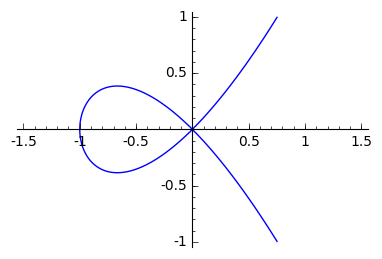
\includegraphics{pics/node.png}
\caption{The nodal curve.}
\end{center}
\end{figure}

We begin by mapping each point of the curve, except the origin, into a three dimensional space via the map that sends $(x,y)$ to $(x,y,y/x)$. We note that the $z$-coordinate is just the slope of the direct line connecting the point $(x,y)$ with the origin.

\begin{figure}[!htbp]\label{blownUpNode}
\begin{center}
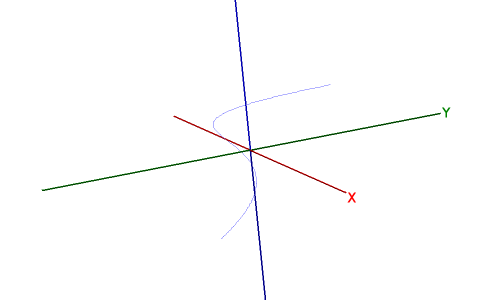
\includegraphics[scale=0.8]{pics/blown_up_node.png}
\caption{The Zariski closure of the image of nodal curve in affine 3-space.}
\end{center}
\end{figure}

When we embed the nodal curve, except of course the origin, this way into the affine three space $\Aff^3$, the resulting space curve won't have any points on the locus $x=0$. The points $(x,y,z)$ belonging to the image satisfy two algebraic relations. First of all, they must satisfy $y^2 - x^3 - x^2 = 0$ for this was the defining equation for the nodal curve. Secondly, we must have $zx = y$ because we sent the point $(x,y)$ of the curve to $(x,y,y/x)$.

Any point of $\Aff^3$ having $x=0$ and $y=0$ satisfy the two algebraic relations we just mentioned, and in fact, if we denote by $C'$ the set of points in $\Aff^3$ lying in the image of the nodal curve without origin, we can see that the two polynomial equations cut out exactly $C'$ and the $z$-axis. This seems to be uneconomic in some sense, and we can actually do better. The \emph{Zariski closure} $\overline{C'}$ of $C'$ in $\Aff^3$ is the smallest subset of $\Aff^3$ that is given by some polynomial equation system and that contains $C'$. In this case it is the set of points cut out by $zx - y$ and $z^2 - x - 1$, and it is visualized in \fref{blownUpNode}. Projection $\Aff ^3 \to \Aff^2$ sending $(x,y,z) \to (x,y)$ maps the Zariski closure $\overline{C'}$ to the nodal curve $C$, and this mapping $\overline{C'} \to C$ is called the \emph{blow-up}.

Outside the origin the preimage of a point of the nodal curve $C$ is a single point in $\overline{C'}$, and the preimage of the origin consist of two points that correspond to the two branches. The blown up curve $\overline{C'}$ contains no singularities, so we have managed to resolve them. In this section, we are going to give the basic constructions and results of blow-ups.

\subsection{Blowing up points in an affine space}

Blowing up a point in an affine space $\Aff^n$ is essentially very similar to what happened at the beginning of this section, although it is a bit more technical. We are only going to describe how to blow up the origin as the technique trivially generalizes to other points as well. From now on, unless otherwise stated, we work over an algebraically closed field.

The basic idea is to replace the origin with $\Proj^{n-1}$ whose points corresponds to all the ''tangent directions'' at 0. We begin by taking the product space $\Aff^n \times \Proj^{n-1}$, whose coordinates we are going to denote by $(x_1,...,x_n, [u_1:...:u_n])$. We would like to have only the points of form $(x_1,...,x_n, [x_1:...:,x_n])$, we set the blown up space $\bl_0 (\Aff^n)$ (where 0 stands for the fact that we blow up the origin) to be the closed subvariety of $\Aff^n \times \Proj^{n-1}$ cut out by equations $x_i u_j - x_j u_i = 0$. The first projection map clearly induces a morphism $\bl_0 (\Aff^n) \to \Aff^n$ that is isomorphism outside the origin of $\Aff^n$. Over the origin we have the whole projective $(n-1)$-space, so we have managed to do exactly what we wanted.

It is however more interesting to see what happens to \emph{subvarieties} $X$ of $\Aff^n$ under the blow-up. The preimage of $X$ in the map $\bl (\Aff^n) \to \Aff^n$ is called the \emph{total transform} of $X$, and it is denoted by $X^{tot}$. The Zariski closure of the preimage of $X \backslash \{ 0 \}$ in $\bl (\Aff^n)$ is called the \emph{strict transform} $X^{st}$ of $X$, and taking the strict transform is what is usually meant when we talk about blowing up $X$. It is clear that the blow-up map $\bl (\Aff^n) \to \Aff^n$ restricts to give morphisms $X^{tot} \to X$ and $X^{st} \to X$.

\begin{ex}
Lets get back to the example of the nodal curve $C$ cut out of $\Aff^2$ by the polynomial $y^2 - x^3 - x^2$. We denote the points of the product variety $\Aff^2 \times \Proj^2$ by $(x,y, [u:v])$, so the blown up plane $\bl (\Aff^2)$ is cut out by the polynomial $xv - yu$. Now the preimage of $C$ in $\bl (\Aff^2)$ is cut out by furthermore requiring the equation $y^2 - x^3 - x^2$ to be satisfied. It is easy to see that if $(x,y) \not =  (0,0)$, then $(x,y,[x:y])$ is the only point of $C^{tot}$ lying over it, and as every point of form $(0,0, [u:v])$ is in $C^{tot}$, we see that the preimage of the origin is the whole $\Proj^1$.

We can compute the strict transform of $C$ locally. We pass to the locus where $u \not = 0$, so that we can parametrize the points by $(x,y,z)$ where $z = v/u$. The part of the blown up plane lying here is cut out by $xz - y$. Now we notice that, as an algebraic variety, this is isomorphic to affine 2-space $\Aff^2$ by the map $(x,z) \mapsto (x,xz,z)$. The preimage of $C$ minus the origin in this latter affine 2-space is the zero set of $x^2 z^2 - x^3 - x^2$ outside the locus $x=0$ (if $x=0$, then also $xz=y$ is 0). The smallest algebraic set containing the preimage is the one cut out by $z^2 - x - 1$, because the resulting algebraic set must be one dimensional, and because the curve defined by the above equation is irreducible. 

We conclude that in the first chart of $\Aff^2 \times \Proj^1$ the strict transform of $C^{st}$ is cut out by the equations $xz - y$ and $z^2 - x - 1$, and hence the equations $xv - yu$ and $v^2 - (x+1)u^2$ almost cut out the strict transform in $\Aff^2 \times \Proj^1$. As there may still be some extra points in the locus $u=0$, we compute the strict transform in the second chart of $\Aff^2 \times \Proj^1$ and see that the equation $1 - y z^{-3} - z^{-2}$. Therefore we obtain one additional equation $v^3 - yu^3 - u^2 v = 0$. Hence the strict transform $C^{st} \subset \Aff^2 \times \Proj^1$ is given by the equations
\begin{align*}
xv - yu &= 0 \\
v^2 - (x+1)u^2 &= 0 \\
v^3 - yu^3 - u^2 v &= 0.
\end{align*}
\end{ex}

\begin{ex}
The procedure given in the last example easily generalizes to computing the strict transformation of a hypersurface $X \subset \Aff^n$ when blowing up the origin. Let $f$ be the defining polynomial for $X$, and let $d$ be the degree of its lowest term. For the $i^{th}$ chart of the $\Aff^{n} \times \Proj^{n-1}$ we get the relations 
\begin{equation*}
x_j = {u_j \over u_i} x_i  
\end{equation*}
and the polynomial $f(x_1,...,x_n)$ transforms into 
\begin{equation*}
f({u_1 \over u_i} x_i, ... ,{u_n \over u_i} x_i) = x_i^d \cdot g({u_1 \over u_i} x_i, ... ,{u_n \over u_i} x_i),
\end{equation*}
where $g$ is not divisible by $x_i$. As the variety in question is isomorphic to $\Aff^{n}$ with coordinates $x_i, u_1/u_i,...,u_n/u_i$, we can again conclude that the Zariski closure in the $i^{th}$ chart is cut out by the polynomial $g$. Therefore one can compute the strict transform $X^{st}$ of the hypersurface $X$ simply by finding the local equations for all the $n$ charts. Finding the strict transform of non-hypersurfaces is harder, as finding the Zariski closure is not as simple, not even locally.
\end{ex}

\begin{ex}
Assume that we have a plane curve $C$, cut out by polynomial $f$, and that the origin is a simple singularity of degree $d$. This means that at the origin we have $d$ branches of the curve meeting transversally, i.e., their tangent lines are distinct. The lowest degree form $F_{min}$ of $f$ factors into a linear product $\prod_i (a_i x_i - b_i y_i)$ and the lines defined by these linear factors are known to be exactly the tangent lines of the branches at the origin. Hence, the degree of the form is $d$, and the linear factors are pairwisely different.

Blowing up this kind of singularity resolves it immediately. We break the polynomial $f$ into a sum $F_d + F_{d+1} + ... + F_n$ of its homogeneous parts, the reader should note that $F_d = F_{min}$. We can see that the polynomial $x^{-d} f(x,xz)$ defining the strict transformation is now 
\begin{equation*}
F_d(1,z) + x F_{d+1} (1,z) + ... + x^{n-d} F_n (1,z),
\end{equation*}
from which we see that the points of the strict transform $C^{st}$ lying over the origin in the first chart are exactly the ones having $x=0$ and $z$ satisfying $F_d(1,z)$, which by assumption splits into \emph{distinct} linear factors. As the intersection multiplicity with $x=0$ is 1 at each of these points, we see that the points must be simple. In the other chart one does exactly the same things, and by symmetry we can conclude that all points lying over the origin in the strict transformation $X^{st}$ are simple.
\end{ex}

\begin{ex}
A single blow-up may not be able to resolve the singularity even in the case of plane curves. Take the curve $y^2 - x^5 = 0$. The strict transform of in the first chart is cut out by $z^2 - x^3$, which has cusp at the origin. This could be resolved by blowing up the origin again (which we strictly speaking don't know how to do yet, because the strict transform is not necessarily contained in a affine space). 
\end{ex}

\begin{ex}
Sometimes we cannot resolve a singular point no matter how many times we blow it up. The famous example of this is the \emph{Whitney umbrella} which is an algebraic surface in $\Aff^3$ cut out by $x^2 - y^2 z$. We compute the strict transform on the $z$-chart with coordinates $x',y',z$ where $x=x'z$ and $x=x'z$, and see that it is cut out by the equation $z^{-2} (x'^2 z^2 - y'^2z^3) = x'^2 - y'^2z$, which is essentially the same equation! Therefore blowing up the origin can never resolve the singularity. The singularity of the Whitney umbrella can however be resolved by blowing up, but instead of blowing up a point, we need to blow up the whole $z$-axis.
\end{ex}

\subsection{Blowing up simple subvarities}

In some cases it is very easy to see what \emph{blowing up a subvariety} $Y$ of $\Aff^n$ should mean. Take for example the $z$-axis $Z$ in $\Aff^3$. We can think about $\Aff^3$ as an infinite family of affine $2$-spaces parametrized by the $z$-coordinate, and we interpret blowing up the $z$-axis (almost) just as blowing up the origin at each of these planes simultaneously. We end up with the blow-up map $\bl (\Aff^n) \times \Aff^1 \cong \bl_Z(\Aff^3) \to \Aff^3$. The strict and total transforms of subvarities are defined similarly as before.

\begin{ex}
We can now resolve the Whitney umbrella, which is cut out by $x^2 - y^2 z$. The coordinates for $\bl_Z (A^3)$ are $(x,y,z,[u:v])$, and the relation $xv-yu = 0$ is satisfied. On the first chart, we have 
\begin{equation*}
y = x {v \over u},
\end{equation*} 
and hence the defining equation can be transformed into
\begin{equation*}
x^2 -  x^2\left( {v \over u} \right)^2 z = x^2 ( 1 - \left( {v \over u} \right)^2 z ).
\end{equation*}
Therefore the first chart gives us the equation $u^2 - v^2 z = 0$. Similarly we can calculate the strict transform in the second chart, but we get exactly the same equation from there. Hence the strict transform of the Whitney umbrella is the closed subvariety of $\Aff^3 \times \Proj^1$ cut out by the equations
\begin{align*}
xv-yu &= 0\\
u^2 - v^2 z &= 0.
\end{align*}
Moreover, we can see from the local equations that the strict transform is nonsingular, so we have managed to resolve the Whitney umbrella.
\end{ex}

\subsection{Blowing up, the general construction}

Let $X$ be a scheme and $\mathscr{I}$ a sheaf of ideals (we require them to be quasicoherent and finite type) on $X$. The \emph{blow-up of $X$ along $\mathscr{I}$}, $\bl_{\mathscr{I}} (X)$, is defined as 
\begin{equation*}
\rproj ( \OO_X \oplus \mathscr{I} \oplus \mathscr{I}^2 \oplus ...),
\end{equation*}
where $\OO_X \oplus \mathscr{I} \oplus \mathscr{I}^2 \oplus ...$ is to be interpreted as a sheaf of graded algebras on $X$. From the basic properties of the global proj, we know that $\bl_\mathscr{I} (X)$ comes together with a canonical projection map $\bl_\mathscr{I}(X) \to X$. If $Y$ is a closed subscheme of $X$ corresponding to a sheaf of ideals $\mathscr{I}$ on $X$, then we define the \emph{blow-up of $X$ along $Y$}, $\bl_Y (X)$, to be $\bl_\mathscr{I} (X)$.

If $Z \subset X$ is a closed subscheme, then we define the \emph{strict} and the \emph{total transform} of $Z$ under the blow-up $\bl_\mathscr{I}(X) \to X$ or $\bl_Y(X) \to X$ similarly as we did before. 

\begin{ex}
Our new notion coincides with the earlier one. Let's blow up the origin in an affine $n$-space $\Aff_k^n$. The coordinate ring for $\Aff^n$ is just $A = k[x_1,...,x_n]$, and the origin corresponds to the ideal $I = (x_1,...,x_n)$. As we are working over an affine scheme, we only need to show that $\proj (A \oplus I \oplus I^2 \oplus ...)$ naturally corresponds to our earlier notion of blow-up.

Perhaps the easiest way to think about $A \oplus I \oplus I^2 \oplus ...$ is to think it as the Rees-algebra $A[It] \subset A[t]$. This is a quotient of the graded $A$-algebra $A[y_1, ... , y_n]$, where we assume that $y_1,...,y_n$ have no algebraic relations amongst themselves, whose proj is just $\Proj_{\Aff^n}^{n-1}$, which in turn is naturally isomorphic to $\Aff^n \times_k \Proj_k^{n-1}$. Hence it is a closed subscheme of $\Aff^n \times_k \Proj_k^{n-1}$, as was our original definition.

What are the relations we must introduce between $y_i$ in order to get the Rees-algebra $A[It]$? At least we must have $x_i y_j - x_j y_i = 0$, which are exactly the relations that cut the blow-up of our original definition. But are these relations enough this time? As it turns out, they really are, but proving this is a bit tricky.

Every polynomial $f \in A[y_1,...,y_1]$ can be broken into a sum
\begin{equation*}
\sum_i c_i M_i(x_1,...,x_n)N_i(y_1,...,y_n),
\end{equation*}
where $c_i \in k$, and $M_i, N_i$ are monomials. Image of each such term in $A[It]$ is of form
\begin{equation*}
c M(x_1,...,x_n)N(x_1,...,x_n)t^{\deg (N)},
\end{equation*}
which is a monomial in $A[It] \subset k[x_1,...,x_n,t]$. For each such monomial in $A[It]$ we may collect all the summands whose image corresponds to the same monomial up to multiplication by a scalar in $k$. All such terms are of form $c' M'(x_1,...,x_n)N'(x_1,...,x_n)$ such that
\begin{equation*}
M'(x_1,...,x_n)N'(x_1,...,x_n)t^{\deg (N')} = M(x_1,...,x_n)N(x_1,...,x_n)t^{\deg (N)},
\end{equation*}
so if we form the sum of all these, we see that we obtain a polynomial $F$ that is homogeneous as an element of $A[y_1,...,y_n]$ and has as coefficients monomials of $A = k[x_1,...,x_n]$. Moreover, it is also homogeneous as a polynomial in $k[x_1,...,x_n,y_1,...,y_n]$.

Assume now that $f$ is a nonzero polynomial in the kernel of $A[y_1,...,y_n] \to A[It]$. Take some $F$ formed by the above-mentioned procedure. We note that $F$ must lie in the kernel as well, as different monomials in $A[It]$ are linearly independent, and the sum of all coefficients $c' \in k$ preceding the terms of the sum must be 0. We are done if we can show that $F$ is zero modulo the relations $x_i y_j - x_j y_i$. But this is almost trivial. Using the relations $x_i y_j - x_j y_i$ we may transform all the terms in $F$ into some scalar $c'$ times $M(x_1,...,x_n)N(y_1,...,y_n)$. As the sum of the scalars must be 0, the sum thus obtained will be 0, and we are done.

A similar result holds in more general settings, which we are going to prove when we start talking about \emph{smooth blow-ups}. The proof of the more general result is a bit more technical and it uses the theory of Gröbner bases. 
\end{ex}

If we blow up $X$ along an ideal sheaf $\mathscr{I}$ (along a subscheme $Y$) then nothing changes outside the cosupport of $\mathscr{I}$ (outside $Y$).

\begin{prop}
Let us have a sheaf of ideals $\mathscr{I}$ of a scheme $X$, and let $U = X \backslash \cosupp (\mathscr{I})$. Now $U$ is isomorphic to its preimage in the blow-up map. 
\end{prop}
\begin{proof}
Outside the cosupport of $\mathscr{I}$ are exactly the points around which we have a neighbourhood $V$ such that $\mathscr{I} |_V  = \OO_X |_V$, and therefore $\mathscr{I}|_U = \OO_U$. Hence, it is enough to prove that the blow-up of a scheme $X$ along $\OO_X$ is $X$. But this is trivial when we look at the situation locally. If $A$ is a ring, then the Rees-algebra $A[At]$ is just $A[t]$, and hence $\proj (A[t]) = \spec (A)$ naturally along the projection map. As these local projection maps glue to give the global projection map, we are done.
\end{proof}

For any morphism $f: X \to Y$ of schemes and every ideal sheaf $\mathscr{I} \subset \OO_Y$ we have the \emph{inverse image ideal sheaf} $f^{-1} \mathscr{I} \cdot \OO_X$, which is the subsheaf of $\OO_Y$ locally generated by the images of elements of $\OO_Y (U)$ in $\OO_X (f^{-1} U)$. It is not \emph{a priori} clear that this satisfies our definition of an ideal sheaf, as we still need to make sure that it is finitely generated and quasicoherent.

\begin{prop}
The sheaf $f^{-1} \mathscr{I} \cdot \OO_X$ is quasicoherent and finitely generated.
\end{prop}
\begin{proof}
Let $U \subset Y$ and $V \subset f^{-1}U$ be affine open subschemes of $Y$ and $X$ respectively. Now the restriction of $f^{-1} \mathscr{I} \cdot \OO_X$ is clearly generated by the image of $\mathscr{I}|_U$ in the map of rings $\OO_Y (U) \to \OO_X (V)$. Hence, locally, $f^{-1} \mathscr{I} \cdot \OO_X$ is quasicoherent and finitely generated, and we are done.
\end{proof}

An interesting property of the blow-up $\bl_\mathscr{I} (X) \to X$ along $\mathscr{I}$ is the fact that the inverse image sheaf of $\mathscr{I}$ is an invertible sheaf, i.e., locally it is generated by a single nonzerodivisor.

\begin{prop}
The inverse image sheaf of $\mathscr{I}$ under the blow-up map $\bl_\mathscr{I} (X) \to X$ is invertible.
\end{prop}
\begin{proof}
By checking over all affine open $U \subset X$ we see that the ideal in question is the one given the subsheaf 
\begin{equation*}
\mathscr{I} \oplus \mathscr{I}^2 \oplus \mathscr{I}^3 ... \subset \OO_X \oplus \mathscr{I} \oplus \mathscr{I}^2 ... 
\end{equation*}
But the sheaf on $\bl_\mathscr{I} (X)$ given by this graded sheaf is exactly the first twisting sheaf $\OO_{\bl_\mathscr{I} (X)}(1)$, which is known to be invertible. This proves the claim.
\end{proof}

Moreover, blowing up along an invertible ideal sheaf doesn't change anything, so after we blow up along $\mathscr{I}$, then blowing up along the inverse image ideal sheaf does nothing.

\begin{prop}
Let $\mathscr{I}$ be an invertible sheaf of ideals on a scheme $X$. Now the blow-up morphism $\bl_{\mathscr{I}} (X) \to X$ is an isomorphism.
\end{prop}
\begin{proof}
Again, we only need to check this locally. For any open affine $U \subset X$ small enough that $\mathscr{I}|U = I$ is principal and generated by a nonzerodivisor $a \in \OO_U = A$, we see that the Rees-algebra $A[It] = A[at]$ is isomorphic to $A[t]$, reducing us to the case where $I=A$ already solved earlier.   
\end{proof}

The preimage of the cosupport of $\mathscr{I}$ in the blow-up map $\bl_{\mathscr{I}} (X) \to X$ is called the \emph{exceptional divisor} of $\bl_{\mathscr{I}} (X)$. As it is the subscheme cut out by the inverse image ideal sheaf of $\mathscr{I}$, it is truly a divisor, so the name is justified. Moreover, as the sheaf of ideals is locally generated by a single nonzerodivisor, dividing by it does make sense. 

\subsection{Transformations of sheaves of ideals}

In this section we give the definitions for all the different transformations of ideal sheaves under blow-ups we are going to need. Let us have a scheme $X$ and a blow-up map $\bl_{\mathscr{I}}(X) \to X$ along $\mathscr{I}$, and let $\mathscr{J}$ be an ideal sheaf. There are four ways to transform the ideal $\mathscr{J}$ under blow-up:

\begin{itemize}
\item The \emph{total transform} $\mathscr{J}^{tot}$ of $\mathscr{J}$ is just the inverse image ideal sheaf under the map $\bl_{\mathscr{I}}(X) \to X$.

\item The \emph{strict transform} $\mathscr{J}^{st}$ of $\mathscr{J}$ is the ideal sheaf locally generated by images of elements of $\OO_X (U)$ in $\OO_{\bl_{\mathscr{I}}(X)}(U')$, where $U'$ is the preimage of $U$, each divided by the inverse image ideal sheaf of $\mathscr{I}$ as many times as they are divisible by it.

This clearly corresponds to the closure (in the algebro-geometric sense) of the closed subscheme defined by $\mathscr{I}^{tot}$ minus the exceptional divisor in $\bl_{\mathscr{I}} (X)$, and is therefore at least quasicoherent. Over locally Noetherian schemes, however, it is also necessarily finitely generated, and as all schemes we actually work with are locally Noetherian, we see that this is an ideal sheaf.

\item The \emph{weak transform} $\mathscr{J}^{w}$ is the inverse image ideal sheaf of $\mathscr{J}$ under $\bl_{\mathscr{I}}(X) \to X$ divided as many times by the ideal sheaf of the exceptional divisor as possible.

\item The \emph{controlled transform} $\mathscr{J}^{c}$ is like the weak transform except we have the \emph{control} (a positive integer) which limits the number of times we divide by the inverse image ideal sheaf of $\mathscr{I}$.
\end{itemize}

We also have the corresponding transforms for closed subschemes $Y$ of $X$ defined in the obvious way.

\subsection{Isomorphism results}

From our construction of blow-up it is trivial to see that it commutes with passing to an open subscheme, and this also works in the limit, i.e., when restricting to the localization at a point. Next we show that blowing up commutes with passing to a closed subscheme.

\begin{prop}\label{BlowUpCommutesWithClosedEmbeddings}
Let $X$ be a scheme, $\mathscr{I}$ a sheaf of ideals, and let $Y \stackrel{i}{\hookrightarrow} X$ be a closed embedding corresponding to an ideal sheaf $\mathscr{J}$. Now there is a unique morphism $\bl_{\mathscr{I}|_Y}(Y) \to \bl_{\mathscr{I}}(X)$ making the square
\begin{center}
\begin{tikzpicture}[scale=1]
\node (Y) at (0,0) {$Y$};
\node (X) at (3,0) {$X$};
\node (BlY) at (0,2) {$\bl_{\mathscr{I}|_Y}(Y)$};
\node (BlX) at (3,2) {$\bl_{\mathscr{I}}(X)$};
\path[]
(Y) edge[right hook->] (X)
(BlX) edge[->] (X)
(BlY) edge[->] (BlX)
(BlY) edge[->] (Y)
;
\end{tikzpicture}
\end{center}
commute. Moreover, this map is a closed embedding.
\end{prop}
\begin{proof}
It is enough to show this affine-locally, as by uniqueness the local maps must glue to give a global one. So assume that $X = \spec (A)$, and that $Y = \spec (A/J)$. Now the blow-ups correspond to the Rees-algebras $A[It]$ and $(A/J)[\bar{I}t]$, where $\bar I$ is the image of $I$ in $A/J$. There is the natural surjection of graded algebras $A[It] \to (A/J)[\bar{I}t]$ which defines a closed immersion $\bl_{\bar{I}} (Y) \to \bl_I (X)$, so we are left with the task of showing its uniqueness.

The uniqueness is easy to see locally on $\proj (A[It])$. The requirement of commutativity ensures us that for any element $a$ in $A$ or any of its localization is uniquely determined. Let $a_1,...,a_r$ generate $I$, $a \in I$ and let's look at $\OO_{\proj (A[It])} (D(at)) = (A[It]_{at})_0$. Its elements are of form
\begin{equation*}
{F(a_1t,...,a_rt) \over a^dt^d} = {F(a_1,...,a_r) \over a^d},
\end{equation*}
where $F$ is a homogeneous polynomial of degree $d$. Hence all the elements in $(A[It]_{at})_0$ lie in a localization of $A$, and their images are therefore uniquely determined. Therefore there is an unique morphism $\bl_{\bar{I}} (Y) \to \bl_I (X)$ over the map $Y \to X$, so we are done.
\end{proof}

Similar result holds for the other direction.

\begin{prop}
Let $X$ be a scheme, and let $Y \stackrel{i}{\hookrightarrow} X$ be a closed embedding. Let $\mathscr{J}$ be an ideal sheaf on $Y$. Now there is an unique morphism $\bl_{\mathscr{J}}(Y) \to \bl_{i_*\mathscr{J}}(X)$ making the square
\begin{center}
\begin{tikzpicture}[scale=1]
\node (Y) at (0,0) {$Y$};
\node (X) at (3,0) {$X$};
\node (BlY) at (0,2) {$\bl_{\mathscr{J}}(Y)$};
\node (BlX) at (3,2) {$\bl_{i_*\mathscr{J}}(X)$};
\path[]
(Y) edge[right hook->] (X)
(BlX) edge[->] (X)
(BlY) edge[->] (BlX)
(BlY) edge[->] (Y)
;
\end{tikzpicture}
\end{center}
commute. Moreover, this map is a closed embedding.
\end{prop}
\begin{proof}
Now $(i_*\mathscr{J})|_Y = \mathscr{J}$, so this immediately follows from the last proposition.
\end{proof}

Finally, we note that blowing up is independent of the coordinate field.

\begin{prop}
Let $X$ be a $k$-scheme, $\mathscr{I}$ be an ideal sheaf, and let $K$ be a field extension of $k$. Now $\bl_{\mathscr{I}} (X_K)$ is naturally isomorphic to $\bl_{\mathscr{I}} (X)_K$, where the lower index $K$ denotes the extension of scalars $K / k$.
\end{prop}
\begin{proof}
Pass to affine local neighbourhood $\spec (A)$. Locally the blow-up is given by $\proj (A[It])$. Now we have a natural inclusion of graded rings
\begin{equation*}
A [I t] \hookrightarrow (K \otimes_k A) [(K \otimes_k I) t]
\end{equation*}
which induces a map
\begin{equation*}
\proj ((K \otimes_k A) [(K \otimes_k I) t]) \to \proj (A [I t])
\end{equation*} 
of projective schemes. This clearly induces a natural local isomorphism
\begin{equation*}
\proj ((K \otimes_k A) [(K \otimes_k I) t]) \to \spec (K)  \times_{\spec (k)} \proj (A [I t])
\end{equation*}
which glue to give the desired natural isomorphism.
\end{proof}

\subsection{Smooth blow-ups}

An important special case of blow-up is the case when $X$ is a non-singular scheme, $Y \subset X$ a non-singular closed subscheme, and we blow up $X$ along $Y$. In this situation, we say that the blow-up is \emph{smooth}. This special case is the only case necessary for the resolution theorem, and the advantage of restricting our attention to these, is the fact that they are fairly easy to handle. We assume that all non-singular schemes are locally Noetherian.

Localized at a point $p \in Y$, $Y_p$ is cut out by $X_p$ by $r$ equations $a_1,...,a_r \in \OO_{X,p}$ such that $a_1,...,a_r$ is a subsequence for some regular system of parameters. Therefore we can conclude that $a_1, ..., a_r$ form a regular sequence, and that they are prime elements of $\OO_{X,p}$. Hence in some affine open neighbourhood $U$ of $p$, the local sections $a_1,...,a_r \in \OO_X(U)$ form a regular sequence, and each $a_i$ is a prime element. Especially, we can conclude that $a_i$ are distinct prime elements. This leads to our first result concerning the structure of smooth blow-ups.

\begin{prop}\label{StructureOfSmoothBlowUps1}
Let $A$ be a Noetherian integral domain, let $a_1,...,a_r$ be distinct prime elements of $A$ and let $I$ be the ideal generated by the $a_i$. Now the Rees-algebra $A[It]$ is isomorphic to $A[x_1,...,x_r]$, modulo the relations $a_i x_j - a_j x_i = 0$, through the map that sends $x_i$ to $a_i t$. 
\end{prop} 
\begin{proof}
We are interested in finding the relations between the generators of the $A$-algebra $A[a_1 t, ..., a_r t]$. To do this, we will use the theory of Gröbner bases and especially how they relate to elimination theory.

Let us have an $A$-algebra $A[t,x_1,...,x_r]$, and let us order its monomials using the lex-order where we give the greatest significance to $t$, and the least to $x_r$. Consider the ideal $J \subset A[t, x_1,...,x_r]$ generated by $a_i t - x_i$. Its intersection with the subring $A[x_1,...,x_r]$ is exactly the kernel of the surjective map of rings $A[x_1,...,x_r] \to A[It]$ sending $x_i$ to $a_i t$. If we can find a Gröbner basis for $J$ in our chosen monomial order, then we obtain a Gröbner basis for $J \cap A[x_1,...,x_r]$ by taking only the basis elements where we have no $t$.

I claim that one Gröbner basis for $J$ is given by $(a_i t - x_i)_i$ and $(a_i x_j - a_j x_i)_{i,j}$. To prove this, we only need to verify that the Buchberger's criterion holds. It is well know that we do not need to consider the pairs whose leading terms have no nontrivial common factors (here is the point where we need the fact that $a_i$ are prime, otherwise the theory wouldn't necessarily generalize).

Hence, we have essentially only 3 cases to consider:
\begin{itemize}
\item Pair $a_i t - x_i$, $a_j t - x_j$, which gives us $h = a_j(a_i t - x_i) - a_i (a_j t - x_j)  = a_i x_j - a_j x_i$, which is a basis element itself, so this case is clear. 

\item The pair $a_i x_{j_1} - a_{j_1} x_i$, $a_i x_{j_2} - a_{j_2} x_i$, where $j_1,j_2 < i$, which gives us $h = a_{j_2} x_{j_1} x_i - a_{j_1} x_{j_2} x_i$, which in the division algorithm is reduced to zero when we pick the basis element $a_{j_1} x_{j_2} - a_{j_2} x_{j_1}$. 
 
\item The pair $a_{i_1} x_j - a_j x_{i_1}$, $a_{i_2} x_j - a_j x_{i_2}$, where $j < i_1, i_2$, which gives us $h = a_j a_{i_1} x_{i_2} - a_j a_{i_2} x_{i_1}$. Again, it is easy to see that the division algorithm reduces this to zero if we pick the basis element $a_{i_1} x_{i_2} - a_{i_2} x_{i_1}$. 
\end{itemize} 
As we have found the Gröbner basis, we can conclude that the kernel of our map from $A[x_1, ... , x_r]$ to $A[It]$ is generated by $(a_i x_j - a_j x_i)_{i,j}$, and the claim follows.
\end{proof}

\begin{rem}
Assume that $A$ and $A/I$ are regular rings, and that $I$ is generated by a regular sequence $a_1,...,a_r$. Now we at least have a map of graded rings $A[x_1,...,x_r]/(a_i x_j - a_j x_i)_{i,j} \to A[It]$. As the assumptions of the above propositions hold for $a_i$ at least locally near the points of $V(I)$, and as it is easy to see that the map is isomorphism over $D(I)$, we see that the map is locally an isomorphism, and therefore it is an isomorphism. This means that computing smooth blow ups is very easy to do locally, and that checking the suitability of some open set for easy computations is rather easy.
\end{rem}

\begin{rem}
We can now give another proof for \fref{AssociatedPolynomials} under the assumption of the previous remark. The associated graded ring is exactly the quotient of the Rees-algebra $A[It]$ by the homogeneous ideal generated by the elements of $I$, and as 
\begin{equation*}
A[It] \cong A[x_1,...,x_r]/(a_i x_j - a_j x_i)_{i,j},
\end{equation*}
it is easily seen that the associated graded ring will be just $(A/I)[x_1,...,x_r]$.
\end{rem}

\begin{rem}
It is clear that the procedure used in the proof of \fref{StructureOfSmoothBlowUps1} can be generalized to very general situations when trying to understand the structure of a finitely generated sub $A$-algebra of $A[x_1,...,x_n]/I$ in practice. However, if $A$ is not an UFD, then there are some technical difficulties with Buchberger's criterion, as there may not be just one ''elimination polynomial'' $h$. In the proof above, this wasn't a problem, as every leading term had either a unit or a prime coefficien, but in more general situations we might run into trouble. Once these technical difficulties are settled, however, one would be able to, for example, find a representation for \emph{any} Rees-algebra $A[It]$ as a quotient ring of some $A[x_1,...,x_n]$ in an entirely mechanical fashion, and hence be able to compute (essentially) all blow-ups mechanically.
\end{rem}

Another nice thing about a smooth blow-up $\bl_Y (X) \to X$ is that the blown up space $\bl_Y (X)$ stays non-singular, as the next proposition shows.

\begin{prop}
Let $A$ be a regular ring and let $I \subset A$ be an ideal such that $A/I$ is a regular. Now the projective scheme $\proj (A[It])$ is regular. 
\end{prop}
\begin{proof}
We already know that the points outside the exceptional divisor are regular, as the blow-up morphism is an isomorphism there. As the exceptional divisor $D$ is locally cut out by a single nonzerodivisor, we can see that, if $p \in D$ is regular regarded as a point of $D$, then it will also be regular regarded as a point of the blow-up $\proj (A[It])$, so it suffices to characterize the points of $D$.

Recall that the homogeneous ideal associated to $D$ is $I \oplus I^2 \oplus ...$, and hence the exceptional divisor is given by
\begin{equation*}
\proj (A/I \oplus I/I^2 \oplus I^2 / I^3 \oplus ...), 
\end{equation*}
i.e., it is the projective scheme associated to the associated graded ring $\gr_I (A)$. We may assume that $I$ is cut out by some regular sequence $a_1,...,a_r$, and can therefore conclude using \fref{AssociatedPolynomials} that $\gr_I (A) \cong (A/I)[x_1,...,x_r]$. As $A/I$ is known to be regular, the projective scheme $\proj ((A/I)[x_1,...,x_r])$ must be regular too, and we are done.
\end{proof}

\section{Hironaka's Proof}\label{HirRes}

The purpose of this section is to give an outline for the proof for resolution of singularities. The proof is based on modernized versions of the original proof given by Hironaka in 1964 as exposed in \cite{Cut}, \cite{Hau} and \cite{Kol}. Throughout the section, unless otherwise mentioned, all fields will be of characteristic 0, and all varieties will be over such a field. 

\subsection{Order}

Let $X$ be a locally Noetherian scheme, and $\mathscr{I}$ an ideal sheaf on $X$. The \emph{order} of $\mathscr{I}$ at point $p$ is defined as the maximal $n \in \N$ such that $m_{X,p}^n$ contains $\mathscr{I}_p$. By the Krull intersection theorem such an $n$ always exists. Although the definition is quite simple, the order of an ideal is a very important invariant for resolution, and this section is dedicated to understanding its basic properties, and how it interacts with blowing up. First we note that the order is a ''geometric'' invariant.

\begin{prop}
Assume $A$ is a regular local $k$-algebra with $K = A/m_A$ finite over $k$. Now the multiplicity of an ideal $I \subset A$ equals the multiplicity of $\overline{k} \otimes_k I$ at any closed point of $\overline{k} \otimes_k A$.
\end{prop}
\begin{proof}
As $A$ is regular and $k$ of characteristic $0$, we see that the quotient ring $A / m_A^n$ is just $K [x_1,...,x_d]/(x_1,...,x_d)^n$. Hence, if we denote by $r$ the degree of the extension $K / k$, we see that $(\overline{k} \otimes_k A) / (\overline{k} \otimes_k m_A)^n$ is just the product of $r$ copies of $\overline{k}[x_1,...,x_d] / (x_1,...,x_d)^n$. The localization of $(\overline{k} \otimes_k m_A)^n$ at any of the closed points coincides with the $n^{th}$ power of the corresponding maximal ideal, and therefore we see that if $\overline{I} = \overline{k} \otimes_k I \not\subset (\overline{k} \otimes_k m_A)^n$, then the order of $\overline{I}$ is smaller than $n$ at \emph{some} closed point of $\spec (\overline{k} \otimes_k A)$. But clearly the ideal $\overline{I} \otimes_k I$ has the same order at all closed points! Now simply noting that $\overline{I} \subset (\overline{k} \otimes_k m_A)^n$ if and only if $I \subset m_A^n$ proves the claim.
\end{proof}

Assume that we have a smooth variety $X$. We know that $\widehat \OO_{X,p}$ is isomorphic to $K[[x_1,...,x_d]]$, where $K$ is the residue field at $p$. This leads to a nice alternative characterization of the order of an ideal sheaf at $p$.

\begin{prop}\label{TrivOrd}
Let $X$ be a smooth variety and let $\mathscr{I}$ be an ideal sheaf on $X$. Now the order of $\mathscr{I}$ at a point $p \in X$ coincides with the lowest order of any term of any series in
\begin{equation*}
\widehat{\mathscr{I}}_p \subset \widehat \OO_{X,p} = K[[x_1,...,x_d]].
\end{equation*}
\end{prop}
\begin{proof}
This is clear.
\end{proof}

For a $k$-variety $X$, denote by $\der_k(X)$ the (clearly quasicoherent) sheaf of $k$-derivations $\OO_X \to \OO_X$, which by definition is just the dual sheaf of $\Omega_{X/k}$. This sheaf comes with the natural derivation map $\der_k (X) \times \OO_X \to \OO_X$, which is $k$-bilinear. For an ideal sheaf $\mathscr{I} \subset \OO_X$, define its \emph{derivative} $D(\mathscr{I})$ by taking the ideal sheaf locally generated by the local images of $\der_k (X) \times \mathscr{I}$ under the derivation map. This is clearly an ideal sheaf. We can define \emph{higher ideal derivatives} $D^n(\mathscr{I})$ in the obvious way by composing $D$ with itself. We can define $\der_k(A)$ and $D^n (I)$ for a $k$-algebra $A$ and an ideal $I$ in an obvious way.

Assume that $X$ is a smooth $k$-variety. We want to show that the order of $\mathscr I$ is \emph{upper semi-continuous}, i.e., that for each $n \in \N$, the set consisting of points $p \in X$ such that the order of $\mathscr I$ at $p$ is at least $n$, is closed.  Having order $\geq 1$ is equivalent to vanishing, and therefore the claim holds at least for $n=1$. If we can show that the ideal differentiation operator $D$ drops the order by exactly $1$ at all points having nonzero order, then the claim follows easily. This is exactly the strategy we are going to use, although the full proof requires some effort. We begin with a proof for closed points.

\begin{lem}\label{derivativeAtClosedPoints}
Let $X$ be a smooth $k$-variety, and let $\mathscr{I}$ be an ideal sheaf on $X$. Now the order of the derivative ideal $\der_k (\mathscr{I})$ is exactly one smaller than the order of $\mathscr{I}$ at all closed points of $X$ where $\mathscr{I}$ had a nonzero order.
\end{lem}
\begin{proof}
Let $p \in X$ be a closed point, and  let $f_1,...,f_d$ be a regular system of parameters for $\OO_{X,p}$. As the sheaf of relative differentials $\Omega_{X/k}$ over $k$ is locally free of rank $d$, its stalk at $p$ is free of rank $p$. It is well known that the differentials $df_1, ..., df_r$ generate the relative differentials at $p$. As $\Omega_{\OO_{X,p}/k}$ is a free $\OO_{X,p}$-module of rank $r$ by the smoothness assumption, we see that the $df_i$ not only form a generating set, but also a basis as well.

Now we can find differentiation operators $\partial_1,...,\partial_r$ satisfying $\partial_i f_j = \delta_{ij}$. As the completed local ring at $p$ is just the ring of formal power series in $f_i$ over $K$, we see that the $k$-derivate of the ideal $I$ generates an ideal in $K [[f_1,...,f_r]]$ which exactly coincides with the ''usual'' derivative of the ideal generated by $I$ in $K [[f_1,...,f_r]]$. This proves the claim by \fref{TrivOrd}, as the normal differentiation drops the order by one.
\end{proof}

The proof for general points is fairly similar to the proof above, but it requires some additional results concerning differentials.

\begin{prop}
Let $k$ be a field of characteristic 0, and $K/k$ a field extension of transcendence degree $r$. If $\alpha_1, ..., \alpha_r$ is a transcendence basis for $K$ over $k$, then the differentials $d \alpha_1,...,d \alpha_r$ generate the module of relative differentials $\Omega_{K/k}$.
\end{prop}
\begin{proof}
See \cite{Ma} Theorem 59 (27.B).
\end{proof}

Equipped with this result, we can find a basis for the sheaf of relative differentials over a smooth $k$-variety $X$ at generic points.

\begin{lem}
Let $\eta$ be a point of a smooth $k$-variety $X$. If $x_1,...,x_r$ is a regular system of parameters for $\OO_{X,\eta}$, and $[x_{r+1}],...,[x_n]$ a transcendence basis for the residue field $\kappa(\eta)$ over $k$, then the differentials $dx_1,...,dx_n$ form a basis for $\Omega_{X/k}$ at $\eta$.
\end{lem}
\begin{proof}
As $n-r$ is just the dimension of $\overline{\{\eta\}} \subset X$, which is cut out a (locally) regular sequence $x_1,...,x_r$, we see that the dimension of $X$ is exactly $n$. Hence $\Omega_{X/K,\eta}$ is a free $\OO_{X,\eta}$-module of rank $n$, and it is enough to show that $dx_i$ generate it.

By Nakayama's lemma it is enough to show that $dx_i$ generate $\Omega_{X/K,\eta} \otimes_{\OO_{X,\eta}} \kappa (\eta)$. But as the latter module modulo the image of $dx_1,...,dx_r$ can be naturally identified with $\Omega_{\kappa(\eta) /k}$, the claim follows from the previous proposition. 
\end{proof}

We are now ready to prove that the order drops exactly by $1$ all points with nonzero order.

\begin{prop}
Let $X$ be a smooth $k$-variety, and let $\mathscr{I}$ be an ideal sheaf on $X$. Now the order of the derivative ideal $\der_k (\mathscr{I})$ is exactly one smaller than the order of $\mathscr{I}$ at all points $\eta$ of $X$ where $\mathscr{I}$ had a nonzero order.
\end{prop}
\begin{proof}
Let $x_1,...,x_r$ be a regular system of parameters for $\OO_{X,\eta}$, and $[x_{r+1}],...,[x_n]$ a transcendence basis for $\kappa(\eta)/k$. By the previous proposition, $dx_i$ form a basis for the module of relative differentials at $\eta$, and therefore we can find differential operators $\partial_1,...,\partial_n$ satisfying $\partial_i x_j = \delta_{ij}$. Again, as in the proof of \fref{derivativeAtClosedPoints}, it is clear that if we look at the ideal generated by the image of $\mathscr{I}_\eta$ under the differential operators $\partial_1,...,\partial_r$, it is clear that the order of the resulting ideal is exactly one smaller than before differentiating. After all, the completed local ring at $\eta$ is just the ring of formal power series in $x_1,...,x_r$ over $\kappa(\eta)$, and the order coincides exactly with the usual order of the latter ring. But as $\partial_{r+1},...,\partial_n$ only touch the ''constant coefficients'', we see that the order of any function can only increase under these operators, and we are done. 
\end{proof}

As an immediate corollary, we obtain the following theorem:

\begin{thm}
\textbf{Upper semi-continuity of order.} Let $X$ be a smooth $k$-variety, $\mathscr{I}$ an ideal sheaf. Denote by $\nu_{\mathscr{I}}$ the function $X \to \N$ sending a point $p$ in $X$ to the order of $\mathscr{I}$ at $p$. Now the function $\nu_\mathscr{I}$ is upper semi-continuous, i.e., for each $n \in \N$ the set consisting of $p \in X$ such that $\nu_\mathscr{I} (p) \geq n$ is closed. 
\end{thm}
\begin{proof}
This is clear for $n=1$, and for higher $n$ the claim follows by differentiating $\mathscr{I}$.
\end{proof}

As $\mathscr I$ has finite order at all points of $X$, and as $X$ is a Noetherian topological space, we see that there is some highest $n \in \N$ such that $X$ has points where the order of $\mathscr{I}$ is at least $n$. The collection of all such points -- \emph{the top locus} of $\mathscr I$ -- is a closed subset of $X$ denoted by $\mathrm{top} (X)$.

\subsubsection*{An algebraic digression -- Zariski's lemma on Holomorphic Functions}

Using the results we have concerning differentiating ideals, we can prove a classical theorem concerning orders of vanishing. Namely

\begin{prop}
\textbf{Zariski's lemma.} Let $X$ be a smooth $k$-variety, $\mathscr{I}$ an ideal sheaf, and $\eta$ some generic point. Now the order of $\mathscr{I}$ at $\eta$ equals the smallest of the orders of $\mathscr{I}$ at closed points $p$ lying in the closure of $\eta$. 
\end{prop}
\begin{proof}
It is known that $I$ vanishes at $\eta$ if and only if it vansishes at all closed points of $\overline{\{\eta\}}$. Using the fact that differentiating $\mathscr{I}$ drops the order by one at all points where the order was nonzero, the claim follows immediately.
\end{proof}

The previous statement can be formulated in a more algebraic fashion. Assume $A$ is a commutative ring, and $I$ is its ideal. Now the order of the ideal $I$ at the point corresponding to a prime ideal $p \subset A$ is clearly the largest $n$ for which $I$ is contained in the $n^{th}$ symbolic power $p^{(n)}$ of $p$. Hence we have proven the following algebraic result:

\begin{prop}
Let $A$ be a finitely generated $k$-algebra ($\mathrm{char} (k) = 0$) corresponding to a smooth $k$-variety $\spec (A)$. Let $p$ be a prime ideal of $A$. Now
\begin{equation*}
p^{(n)} = \bigcap_m m^n,
\end{equation*}
where $m$ runs over all the maximal ideals of $A$ containing $p$.
\end{prop}
\begin{proof}
The result is immeadiate once we note that for maximal ideals $m$ the symbolic powers $m^{(n)}$ and the ordinary powers $m^n$ coincide.
\end{proof}

\subsubsection*{Some properties of order}

Assume $X$ is a smooth $k$-variety, and denote the order of an ideal sheaf $\mathscr{I}$ at $p \in X$ by $\nu_p (\mathscr{I})$. Using the characterization of order by the means of formal power series, the following proposition is immediate:
\begin{prop}
Let $\mathscr{I}$ and $\mathscr{J}$ be ideal sheaves on $X$. Now
\begin{equation*}
\nu_p (\mathscr{I} \mathscr{J}) = \nu_p (\mathscr{I}) +  \nu_p(\mathscr{J})
\end{equation*}
and
\begin{equation*}
\nu_p (\mathscr{I} + \mathscr{J}) = \mathrm{min} (\nu_p (\mathscr{I}),  \nu_p(\mathscr{J})).
\end{equation*}
\end{prop}

Next we are interested in how the order of ideals changes in \emph{monomial transforms}, i.e., under blow-ups. More precicely, we are interested how the order of an ideal is affected when we take the weak transformation in some blow up.

\begin{prop}
Let $\mathscr{J}$ be an ideal sheaf on $X$, and let $\mathscr{I}$ be the ideal sheaf of some regular closed subscheme $Y$ of $X$ contained in the top locus of $\mathscr{J}$. Now the maximal order of $\mathscr{J}^w$ on $\bl_{\mathscr{I}} (X)$ is not greater than that of $\mathscr{J}$ on $X$.
\end{prop}
\begin{proof}
By Zariski's main lemma on holomorphic functions, we need to show only that if the order of $\mathscr{J}$ is $o$ at some \emph{closed} point $p$ of $X$, then the order of $\mathscr{J}^w$ at any closed point $p'$ of $\bl_{\mathscr{I}} (X)$ is at most $o$. As both the order of an ideal and blowing up behave well under extension of scalars, we may assume that the coefficient field $k$ is algebraically closed.

We reduce to the local case around some closed (necessarily $k$-valued) point $p \in X$. Nothing interesting happens if $p \not\in V(\mathscr{I})$, so we have a regular local ring $A$, a proper ideal $I \subset A$ generated by a subsequence of some regular system of parameters, and an ideal $J \subset A$. Let $a_1,...,a_n$ be a regular system of parameters of $A$, and $I = (a_1,...,a_r)$. 


We already know that the exceptional divisor of $\bl_I (X)$ is $\proj ((A/I) [x_1,...,x_r])$, and therefore the points of the blow-up that lie over $p$ form the projective scheme $\proj (k[x_1,...,x_r])$. By performing linear transformation on the $a_1,...,a_r$, we may assume that the point on the blown up scheme $\bl_{\mathscr{I}} (X)$ we are interested in corresponds to the point $[1:0:...:0]$ in the projective scheme.

The local blow-up corresponds to the graded algebra $A[a_1 t, ..., a_r t]$, whose first chart is the spectrum of 
\begin{equation*}
A \left[ {a_2 \over a_1}, ... , {a_r \over a_1} \right].
\end{equation*}
The point we are interested in corresponds to the maximal ideal
\begin{equation*}
\left( a_1, {a_2 \over a_1}, ... , {a_r \over a_1} \right).
\end{equation*}
As everything stays smooth and $n$-dimensional, we see that this is also a regular system of parameters for that point. Hence, formally locally, we have a map of rings of formal power series
\begin{equation*}
k[[x_1,...,x_r]] \to k[[y_1,...,y_r]]
\end{equation*}
defined by $x_1 \mapsto y_1$, and $x_i \mapsto y_1 y_i$ for $i>1$.

Hence we can conclude that in \emph{all smooth blow-ups, the order of the total transformation $J^w$ at some point $p'$ is at most twice the order of $J$ at the point $p$ that $p'$ lies over.} Now we just need to see what happens when we divide by the ideal of the exceptional divisor.

On the first chart of the blow-up, we see that the image of $I$ in
\begin{equation*}
A \hookrightarrow A \left[ {a_2 \over a_1}, ... , {a_r \over a_1} \right].
\end{equation*}
is actually generated by $a_1$. Hence dividing an ideal by the ideal of the exceptional locally corresponds to dividing it by $a_1$, and hence each division drops the order by $1$. Also from the formally local characterization, and from the fact that the order of $J$ is $o$ along the whole vanishing set of $I$, we see that we can divide $J^{tot}$ by the inverse image sheaf of $I$ exactly $o$ times (as this is the case at each closed point). This concludes the proof.  
\end{proof} 
 
\subsection{From resolution of singularities to monomialization of ideals} 

A characteristic part of the Hironaka's proof for resolution of singularities is the shift of emphasis from subvarieties to ideal sheaves. Instead of having a closed subvariety $Y$ of a smooth $k$-variety $X$ and looking its transformations in successive blow-ups on $X$, we take the ideal sheaf corresponding to $Y$ and look at its transformations. Although initially this might seem to be just a formal trick (and in some sense it actually is), some notions are far more natural to define for ideal sheaves than they are for subvarieties, and hence this change of perspective is very beneficial.  

An ideal sheaf $\mathscr{I}$ of a smooth $k$-variety $X$ is called \emph{(locally) monomial} if at any point $p$ of $X$, we have a choice of regular system of parameters $x_1,...,x_r$ at $p$ such that the stalk of $\mathscr{I}$ at $p$ is generated by an element of form $x_1^{e_1} x_2^{e_2} \cdots x_r^{e_r}$. The vanishing scheme of a monomial ideal sheaf (which can be thought as a divisor in a natural way) is called a simple normal crossing scheme or a simple normal crossing divisor.

We are getting near to shifting our emphasis and stating our new goal, but we still need to introduce some new terminology and notation. For a birational morphism $g: X' \to X$, denote by $\Ex (g)$ the \emph{exceptional locus of $g$}, i.e., the set of points of $X'$ where $g$ is not a local isomorphism. For blow-ups, this is usually just the exceptional divisor, with the exception of blowing up along an ideal that is generated by a single nonzerodivisor near some point $p$. Exceptional locuses work as one would expect in compositions:

\begin{lem}
Let $g: X' \to X$ and $g': X'' \to X'$ be birational morphisms of (locally) integral schemes. Now we have
\begin{equation*}
\Ex (g \circ g') = \Ex (g') \cup g'^{-1} (\Ex(g)).
\end{equation*}
\end{lem}
\begin{proof}
Let $p'' \in X''$, $p' \in X'$ and $p \in X$ be send to each other by our birational maps. We need to show that the composition
\begin{equation*}
X''_{p''} \to X'_{p'} \to X_p 
\end{equation*}
is an isomorphism if an only if both the maps $X''_{p''} \to X'_{p'}$ and $X'_{p'} \to X_p$ are. But these maps correspond to birational maps of rings $A \to A'$ and $A' \to A''$, which are necessarily inclusions, making the claim trivial.
\end{proof}

For a sequence
\begin{equation*}
\Pi = X_r \stackrel{\pi_{r-1}}{\to} X_{r-1} \stackrel{\pi_{r-2}}{\to} \cdots \stackrel{\pi_1}{\to} X_1 \stackrel{\pi_0}{\to} X_0
\end{equation*}
of blow-up (we denote by $\Pi$ both the map obtained by composition, and the sequence itself)s of smooth $k$-varieties, where $\pi_i$ is the blow-up with the smooth center $Z_i$, we define the \emph{total exceptional set} $\Ex_{tot} (\Pi)$ to be the union of preimages of all exceptional divisors in $X_r$, i.e.,
\begin{equation*}
\Ex_{tot} (\Pi) = \bigcup_{i=0}^{r-1} (\pi_i \circ \cdots \circ \pi_{r-1}).
\end{equation*}
Assuming that the centres produce nontrivial blow-ups (they are of codimension of at least 2), this equals just the exceptional locus of $\Pi$. For a divisor $E$, define its total exceptional set (again, a divisor) to be  
\begin{equation*}
\Pi_{tot}^{-1} (E) = \Pi^{-1} (E) + \Ex_{tot} (\Pi).
\end{equation*}
This divisor is sometimes also called the \emph{total transform of $E$}.

For a simple normal crossing divisor $E$ and a (necessarily regular) subvariety $Z$ of $Y$, we say that \emph{$Z$ has simple normal crossings with $E$} if at any point of $X$ we can choose local regular parameters $x_1,...,x_n$ such that, locally at points of $Z$, $E = V(x_1^{e_1} \cdots x_n^{e_n})$ and $Z = V(x_1,...,x_r)$. We say that the centres $Z_i$ for the blow-up sequence $\Pi$ \emph{have simple normal crossings with $E$} if for each $i$, $Z_i$ has simple normal crossings with $(\pi_0 \circ \cdots \circ \pi_{i-1})_{tot}^{-1} E$.

Our goal will be to use successive smooth blow-ups to turn an ideal of a smooth $k$-variety $X$ into a monomial one. More precisely, we would want to prove the following theorem:

\begin{thm}
Let $X$ be a smooth $k$-variety, $\mathscr{I}$ a sheaf of ideals, and $E$ a simple normal crossing divisor. Now we have a sequence of smooth blow-ups:
\begin{equation*}
\Pi: R_{\mathscr{I},E} (X) = X_r \stackrel{\pi_{r-1}}{\to} X_{r-1} \stackrel{\pi_{r-2}}{\to} \cdots \stackrel{\pi_{0}}{\to} X_0
\end{equation*}
whose centres have simple normal crossings with $E$, and 
\begin{enumerate}
\item The total transformation $\Pi^{tot} (\mathscr{I})$ (defined by taking successive total transformations in our blow-ups) is locally monomial.
\item The map $\Pi$ is an isomorpism over the nonvanishing locus of $\mathscr{I}$.
\item The map $R_{\mathscr{I},E} (X) \to X$ is functoral on smooth morphisms.
\end{enumerate}
\end{thm} 
We won't discuss what is the precise meaning of (2), and won't discuss why it is important for the complete proof. The reason for this is because technically it is fairly demanding, and is not crucial for the main idea of the proof.

Next we sketch how this is related to our original goal, i.e., how we can resolve the singularities of a variety using monomialization of ideals. For simplicity, we deal only with projective varieties.

\begin{cor}
Let $Y$ be an irreducible projective $k$-variety. Now we have a birational projective morphism $\Pi: R(X) \to X$ such that
\begin{enumerate}
\item $R(X)$ is smooth.
\item $\Pi$ is an isomorphism outside the singular locus of $X$ (which is closed).
\end{enumerate}
\end{cor}  
\begin{proof}
If the dimension of $Y$ is $d$, then we may assume it to be a regular subscheme of $X = \Proj^n_k$, where the difference of dimensions $n-d$ is at least 2. Let $\mathscr{I}$ be the ideal sheaf on $X$ corresponding to $Y$, and let $\Pi$ be a sequence of blow-ups given by the previous theorem. 

As the total transformation $\Pi^{tot} (\mathscr{I})$ is a monomial sheaf, the total transformation of the subvariety $Y$ along the sequence $\Pi$ is of codimension $1$, i.e., its dimension must be strictly larger than that of $Y$. As nothing changes outside the centre of the blowup, we must have some first blow up $\pi_i: X_{i+1} \to X_i$ whose centre $Z_i$ contains the generic point $\eta$ of $Y$.
\end{proof}
 
\subsection{Monomalization of ideals -- an outline of the proof}

\section{de Jong's Proof}\label{deJongRes}

\begin{thebibliography}{5, style=alpha}

\bibitem[AtM]{AtM} 
Michael Atiyah and Ian Macdonald: Introduction to Commutative Algebra, Addison-Wesley.

\bibitem[Cut]{Cut} 
Steven Dale Cutkosky: Resolution of Singularities, Graduate Studies in Mathematics 63, 2004.

\bibitem[Eis]{Eis}
David Eisenbud: Commutative Algebra with a View Toward Algebraic Geometry, Springer-Verlag.

\bibitem[EisHo]{EisHo}
David Eisenbud and Melvin Hochster: A Nullstellensatz with Nilpotents and Zariski's Main Lemma on Holomorphic Functions, Journal of Algebra 58, 1979.

\bibitem[Har]{Har}
Robin Hartshorne: Algebraic Geometry, 1st edition, Springer, 1977.

\bibitem[Hau]{Hau}
Herwig Hauser: The Hironaka Theorem on Resolution of Singularities (Or: A proof we always wanted to understand) Bull. Amer. Math. Soc. 40 (2003).

\bibitem[HLOQ]{HLOQ} 
Hauser, Lipman, Oort, Quirós: Resolution of Singularities - A research textbook in tribute to Oscar Zariski, Progress in Mathematics 181, Birkhäuser Verlag, 2000.

\bibitem[Jong]{Jong}
Aise Johan de Jong: Smoothness, semi-stability and alterations, Publications Mathématiques de l’Institut des Hautes Études Scientifiques (1996).

\bibitem[Kol]{Kol}
János Kollár: Lectures on Resolution of Singularities, Annals of Mathematics Studies 166, 2007.

\bibitem[Ma]{Ma}
Hideyuki Matsumura: Commutative Algebra, W. A. Benjamin, Inc. (1970).

\bibitem[Mum]{Mum}
David Mumford, Selected papers. Volume II. On algebraic geometry, including correspondence with Grothendieck. Springer-Verlag, 2010.

\bibitem[Par]{Par} Carol Parkih: The Unreal Life of Oscar Zariski, Academic Press Inc, 1991.

\bibitem[Ser]{Ser}
Jean-Pierre Serre: Local Algebra, Springer, 2000.

\bibitem[Vak]{Vak}
Ravi Vakil: The Rising Sea - Foundations of Algebraic Geometry.

\bibitem[W\l{}o]{Wlo}
Jaros\l{}aw W\l{}odarczyk: Simple Hironaka Resolution in Characteristic Zero, J. Amer. Math. Soc. 18 (2005)
\end{thebibliography}


\end{document}
